%%%%%%%%%%%%%%%%%%%%%%%%%%%%%%%%%%%%%%%%%%%%%%%%%%%%%%%%%%%%%%%%%%%%%%%%%%%%%%
% Jan Kalina <xkalin03@stud.fit.vutbr.cz> 2014
%%%%%%%%%%%%%%%%%%%%%%%%%%%%%%%%%%%%%%%%%%%%%%%%%%%%%%%%%%%%%%%%%%%%%%%%%%%%%%

%%%%%%%%%%%%%%%%%%%%%%%%%%%%%%%%%%%%%%%%%%%%%%%%%%%%%%%%%%%%%%%%%%%%%%%%%%%%%%
\chapter{Úvod} \label{uplnyUvod}
%%%%%%%%%%%%%%%%%%%%%%%%%%%%%%%%%%%%%%%%%%%%%%%%%%%%%%%%%%%%%%%%%%%%%%%%%%%%%%

Okolo bezpečnosti serverů poskytujících své služby počítačům v~síti bylo již zpracováno mnoho různých prací.
Tato práce se však nezabývá problémem, jak zabránit útoku zvenčí útočníkům v~síti, ale jak předejít nebezpečí ze strany aplikací nainstalovaných na tomto serveru.
Zabývá se tedy tím, jak omezit možnosti aplikací běžících v~daném systému a zabránit jim v~přístupu ke zdrojům systému, na které nemají nárok.

Tato omezení mohou plnit různé účely -- od zabránění vzájemnému přístupu k~datům jedné aplikace druhou aplikací jiného provozovatele,
v~rámci serveru sdíleného mezi více provozovateli aplikací, po zabránění škodám na jiných aplikacích a službách v~případě úspěšného prolomení
zabezpečení jedné z~aplikací běžících na serveru sdíleného více aplikacemi.

Pro podobné účely se obvykle využívají oprávnění na úrovni operačního systému.
Ty však, ať už se jedná o~jednoduchá unixová oprávnění, podrobnější NTFS oprávnění, či ještě podrobnější oprávnění systému SELinux,
nejsou schopny rozlišit jednotlivé aplikace běžící v~rámci jediného procesu.
Takovým procesem, v~rámci něhož může běžet více aplikací, je například aplikačního server WildFly.

Tento problém je možné vyřešit na úrovni virtuálního stroje Javy, uvnitř kterého aplikační server běží, za pomoci tzv. správce bezpečnosti (Security Manager)
a bezpečnostních politik (Security Policy). Ty umožňují omezovat oprávnění kódu jednotlivých tříd v~Javě.
Jejich obecné použití je podrobně popsáno v~kapitole \ref{teoretickyUvod}, jejich použitím v~rámci aplikačního serveru WildFly se pak zabývá kapitola \ref{jboss}.

V~prostředí datových center jsou aplikační servery spojovány do centrálně spravovaných distribuovaných prostředí, takzvaných domén.
V~tomto prostředí se může jako velmi užitečná projevit možnost centrální správy těchto bezpečnostních politik napříč servery této domény.

Řešení umožňující centrální správu bezpečnostních politik je hlavním tématem této bakalářské práce.
Je implementováno jako rozšíření aplikačního serveru WildFly a jeho webové uživatelské rozhraní jako rozšíření webové administrační konzole WildFly.
Jeho návrh je nastíněn v~kapitole \ref{navrh}, jeho implementace je popsána v~kapitole \ref{implementace} a jeho testování v~kapitole \ref{testovani}.

Implementace tohoto řešení byla úspěšná a výsledkem této práce je tedy rozšíření WildFly, umožňující využívat a za běhu aplikačního serveru
nastavovat soubory bezpečnostní politiky Javy.
Je tak přímo uplatnitelné ve stávajících aplikacích aplikačního serveru WildFly, kde je kladen velký důraz na bezpečnost.

%%%%%%%%%%%%%%%%%%%%%%%%%%%%%%%%%%%%%%%%%%%%%%%%%%%%%%%%%%%%%%%%%%%%%%%%%%%%%%
\chapter{Bezpečnost v~Javě} \label{teoretickyUvod}
%%%%%%%%%%%%%%%%%%%%%%%%%%%%%%%%%%%%%%%%%%%%%%%%%%%%%%%%%%%%%%%%%%%%%%%%%%%%%%

%=============================================================================
\section{Bezpečnost}
%=============================================================================

Protože se tato práce zabývá bezpečností, což je pojem, který lze v~různých souvislostech chápat zcela odlišně. Je nanejvýš vhodné nejprve specifikovat co termínem bezpečnosti míníme a z~jakého pohledu se jí budeme zabývat.

Scott Oaks definuje ve své knize Java Security bezpečnost jako souhrn následujících kritérií: \cite{oaks}

\begin{itemize}
  \item {\bf Bezpečí vůči zákeřnému software} -- programy by neměly být schopny poškodit prostředí hostitelského počítače.
  \item {\bf Bezpečí vůči Velkému bratru} -- programům by mělo být bráněno ve sledování uživatele -- programy by neměly být schopny svévolně číst soukromé informace na počítači, na kterém běží, ani na síti, ke které je tento počítač připojen.
  \item {\bf Autentizace} -- identita autorů programu by měla být ověřována (typicky pomocí digitálního podpisu).
  \item Šifrování -- data odesílaná a přijímaná programem by měla být šifrována.
  \item Auditovatelnost -- potenciálně škodlivé operace by měly být vždy zaznamenávány.
  \item Specifikovanost -- program by měla doprovázet specifikace bezpečnostních pravidel, které program dodržuje.
  \item Verifikovanost -- pro prováděné operace by měla být stanovena pravidla, proti kterým by měly být verifikovány.
  \item Dbaní na dobré vychování -- programům by mělo být bráněno v~užívání příliš mnoha systémových prostředků.
\end{itemize}

V~souvislosti s~víceuživatelskými prostředími se pak pojem bezpečnosti vyskytuje ještě v~další rovině, kdy nejde o~bezpečí systému před běžící aplikací, ale o~způsob jakým může naopak program ověřit, kdo je jeho uživatelem a zdali má právo po něm žádat vykonání operace, o~jejíž vykonání žádá. Touto stránkou bezpečnosti se však tato práce zabývat nebude.

Tato práce se zabývá bezpečností ve smyslu prvních tří bodů uvedeného výčtu (zvýrazněny tučně). Bude se tedy zabývat způsobem ochrany prostředí hostitelského počítače před jeho poškozením nebo neoprávněným sledováním ze strany běžících programů. Právě oprávnění programu pak souvisí s~autentizací. Autentizací se myslí ověřování autorství programu. Právě od toho, kdo je autorem programu, se totiž mohou oprávnění programu často odvozovat.

%=============================================================================
\section{Java}
%=============================================================================

Programy v~jazyce Java bývají překládány do platformě nezávislého a efektivně interpretovatelného mezikódu, takzvaného bajtkódu.
Bajtkód (bytecode) bývá zpravidla interpretován virtuálním strojem Javy (JVM - Java Virtual Machine).
\cite{jvmIntro}

JVM je abstraktní výpočetní stroj. Podobně jako reálné výpočetní stroje má svoji instrukční sadu a paměť, se kterou může manipulovat, ale na rozdíl od nich pro něj neexistuje jeho fyzická implementace, pouze emulovaná implementace softwarová.
\cite{jvmIntro}

To znamená, že její kód není prováděn nativně hardwarem. Je interpretován speciálním programem, interpretem, který je sám zkompilovaný do nativního kódu dané platformy a prováděn jejím hardwarem.
To mimo nezávislosti na platformě přináší také vyšší stupeň abstrakce.
\cite{jvmIntro}

Protože programy v~JVM mohou k~fyzickým zdrojům počítače (např. k~souborům nebo k~síti) přistupovat jen skrze JVM, zablokování takového přístupu ze strany JVM není nikterak složité - JVM stačí odmítnout takový požadavek a interpretovaný program nemá možnost JVM obejít.

%=============================================================================
\section{Správce bezpečnosti v~Javě} \label{securityManager}
%=============================================================================

Pro maximální nastavitelnost omezení kladených na programy běžící ve virtuálních strojích Javy nerozhoduje o~povolení nebo zablokování operace nad zdrojem JVM samotná JVM. Dotazuje se namísto toho speciálního objektu, tzv. správce bezpečnosti. \cite{tutorialsTSM}

Správce bezpečnosti je objektem třídy {\tt java.lang.SecurityManager} nebo její podtřídy.
Třídu, jejíž objekt JVM použije při svém startu jako objekt správce bezpečnosti, lze nastavit skrze konfigurační proměnnou JVM {\tt java.security.manager}. \cite{javaSecurityArch}

Aplikace může referenci na aktuálně používaný objekt správce bezpečnosti získat voláním {\tt System.getSecurityManager()} a vypnout nebo jej vyměnit voláním {\tt System.setSecu rityManager()}. Volání těchto metod je samo chráněno správcem bezpečnosti.
Nehrozí tedy, že by se program neoprávněně zbavil omezení, která na něj správce bezpečnosti uvalil, jeho vypnutím nebo výměnou.
\cite{tutorialsTSM}

\begin{figure}[tbh]
\begin{lstlisting}[caption=Příkazy spouštějící program s~výchozím správcem bezpečnosti, label=smEx]
java -Djava.security.manager HelloWorld
java -Djava.security.manager="" HelloWorld
java -Djava.security.manager=default HelloWorld
java -Djava.security.manager=java.lang.SecurityManager HelloWorld
java -Djava.security.manager=cz.test.TestovaciSM HelloWorld
\end{lstlisting}
\end{figure}

Hodnotu konfigurační proměnné {\tt java.security.manager} při startu JVM je možné nastavit za pomoci k~tomu určeného parametru {\tt -D} příkazu {\tt java}.
Je-li hodnota této konfigurační proměnné stanovena na {\tt default} nebo je-li definována bez uvedení hodnoty
(jak demonstrují první tři řádky ukázky kódu \ref{smEx}), je JVM spuštěna s~výchozím správcem bezpečnosti.
\cite{javaSecurityArch}

Jinou možnou hodnotou této konfigurační proměnné je celý název třídy, jenž má být jako správce bezpečnosti použita.
Tento případ demonstrují poslední dva řádky ukázky kódu \ref{smEx}.
Je tak možné nechat o~oprávněních kódu běžícího v~JVM rozhodovat vlastní podtřídu výchozího správce bezpečnosti.
V~rámci inicializace JVM pak bude vytvořena instance třídy určená zmíněnou konfigurační proměnnou.
Tato instance je vytvářena voláním {\tt Class.newInstance()}, tj. za pomoci jeho neparametrického konstruktoru.

Jestliže se vytvoření objektu správce bezpečnosti nezdaří, skončí celá inicializace JVM výjimkou {\tt java.lang.InternalError} \cite{sourceLauncher} a ke spuštění uživatelského programu tak vůbec nedojde.
Je tedy uplatněn bezpečnostní princip, kdy systém zůstane bezpečný i v~případě poruchového stavu, třebaže na úkor funkčnosti.

%-----------------------------------------------------------------------------
\subsection{Implementace vlastního správce bezpečnosti} \label{vlastniSM}
%-----------------------------------------------------------------------------

V~této podkapitole je ukázán způsob stanovení bezpečnostní politiky vytvořením vlastního správce bezpečnosti.
Jak již bylo uvedeno v~kapitole \ref{securityManager}, správce bezpečnosti je objekt (pod)třídy {\tt java.lang.SecurityManager},
na který JVM, při požadavku na Java API (Application Programming Interface -- rozhraní pro programování aplikací), deleguje rozhodnutí o~povolení nebo nepovolení operace nad zdrojem.

Jakmile se tedy uživatelská aplikace pokusí provést potenciálně nebezpečnou operaci (například se pokusí ukončit JVM voláním {\tt System.exit(0)}),
Java API se dotáže správce bezpečnosti na oprávněnost této operace tím, že zavolá jeho, k~tomu určenou, metodu (v~tomto případě {\tt checkExit(0)}). \cite{oaks}

Správce bezpečnosti pak na základě parametrů tohoto volání rozhodne o~tom, zda operaci zakáže a vyvolá k~tomu určenou výjimku {\tt SecurityException}.
Není-li žádná výjimka vyvolána, považuje se operace za povolenou a je provedena. \cite{oaks}

Bezpečnostní politiku tak můžeme definovat vytvořením vlastní podtřídy třídy {\tt Security Manager}, kde přepíšeme metody rozhodující o~povolení
operací, jejichž oprávněnost chceme stanovit.

Od Javy verze Java 2 (SDK v1.2) je možné používat univerzálnější řešení než přepisovat jednotlivé kontrolní metody.
Od této verze totiž všechny kontrolní metody (jakou je {\tt checkExit()}) delegují své rozhodnutí na metodu {\tt checkPermission()} správce bezpečnosti.
Pro stanovení bezpečnostní politiky tak stačí přepsat tuto jedinou metodu. \cite{refSecurityManager}

Příklad jednoduchého správce bezpečnosti ukazuje kód \ref{TestovaciSM}:

\begin{figure}[tbh]
\begin{lstlisting}[caption=Jednoduchý správce bezpečnosti, label=TestovaciSM]
public class TestovaciSM extends SecurityManager {
	@Override
	public void checkPermission(Permission permission) {
		if(permission instanceof FilePermission){
			throw new SecurityException("Prace se soubory je zakazana!");
		}
	}
}
\end{lstlisting}
\end{figure}

Tento jednoduchý správce bezpečnosti implementuje výše zmíněnou metodu {\tt checkPermission()}.
Ta je volána při každém pokusu o~provedení potenciálně nebezpečné operace.
Je-li oprávnění, které uživatelský kód vyžaduje, třídy {\tt FilePermission} nebo její podtřídy, je vyvolána výjimka, která provedení operace zabrání.

V~rámci vlastní aplikace je možné používání vlastního správce bezpečnosti vyvolat za pomoci dříve zmíněného příkazu {\tt System.setSecurityManager()}:

\begin{figure}[tbh]
\begin{lstlisting}[caption=Nastavení správce bezpečnosti zevnitř JVM, label=setSM]
System.setSecurityManager(new TestovaciSM());
\end{lstlisting}
\end{figure}

Z~vně aplikace pak je možné použití tohoto správce bezpečnosti nastavit při startu JVM obdobně, jak je to popsáno v~kapitole \ref{securityManager}:

\begin{figure}[tbh]
\begin{lstlisting}[caption=Spuštění aplikace se správcem bezpečnosti, label=runWithSM]
java -Djava.security.manager=TestovaciSM HelloWorld
\end{lstlisting}
\end{figure}

Vedlejším efektem existence metod volaných při každém pokusu o~provedení potenciálně nebezpečné operace je také možnost vedení statistik, jaká oprávnění
aplikace nejčastěji využívá. Ty by pak teoreticky mohly být základem pro inteligentního správce bezpečnosti, přidělujícího programu oprávnění
na základě heuristické analýzy.

Z~těchto statistik můžeme zjistit například to, že i v~rámci vykonávání prázdného programu v~Javě (třídy, jejíž metoda {\tt main()} neobsahuje žádný příkaz) je prováděno celkem 29 potenciálně nebezpečných operací.
V~18 případech je příčinou dotazu čtení obsahu konfiguračních proměnných (Property), v~8 případech jde o~manipulaci s~vlákny (Thread) a ve zbývajících 3 případech jde o~čtení souboru spouštěné třídy ({\tt Program.class}). Ve všech případech jde tedy o~operace související se samotnou inicializací JVM.

Pro stanovení bezpečnostní politiky se však tento způsob (vytvoření vlastního správce bezpečnosti) v~současnosti již nepoužívá, ačkoli stále možný je.
Důvodem je, že vyžaduje od správce serveru, na němž aplikace běží, znalosti programování.
Neumožňuje navíc jednoduchým způsobem přidělovat oprávnění v~závislosti na třídě, která se potenciálně nebezpečnou operaci snaží provést.

%=============================================================================
\section{Zavaděče tříd} \label{classloader}
%=============================================================================

Než se dostaneme k~v~současnosti využívanému způsobu stanovování bezpečnostní politiky, pozastavíme se nad tématem zavádění tříd.
Ačkoli se na první pohled může zdát, že toto téma s~bezpečností příliš nesouvisí, opak je pravdou.
Jen a pouze zavaděč tříd (classloader), který třídu do paměti zavádí, totiž může určit původ třídy, od kterého se oprávnění kódu této třídy zpravidla odvozuje.

Zavaděč je objekt odpovědný za načítání tříd a rozhraní v~Javě. Na základně binárního názvu třídy (binary name of class) \cite{binaryNameOfClass}, tedy označení třídy používaného v~bajtkódu (např. {\tt java.lang.String} nebo {\tt java.security.KeyStore\$Builder\$FileBuilder\$1}), se tuto třídu pokusí vyhledat a načíst do paměti. \cite{refClassLoader}

Třída každého zavaděče tříd musí být podtřídou třídy {\tt java.lang.ClassLoader} a musí implementovat metodu {\tt findClass()}. Ta je jádrem celého zavaděče -- provádí samotné vyhledání třídy podle názvu. Jejím výstupem je objekt třídy {\tt java.lang.Class}, představující samotnou třídu. \cite{refClassLoader}

\begin{figure}[tbh]
\begin{lstlisting}[caption=Získávání názvu třídy neznámého objektu, label=getClassName]
Class classOfUnknown = unknown.getClass();
String nameOfClass = classOfUnknown.getName(); // "java.lang.String"
\end{lstlisting}
\end{figure}

Při programování běžných aplikací můžeme objekty tříd využít například při snaze získat název třídy neznámého objektu jako řetězec za běhu aplikace,
jak ukazuje ukázka kódu \ref{getClassName}.

První řádek ukazuje získání objektu třídy (objektu třídy {\tt Class}) neznámého objektu.
To je možné díky tomu, že každý objekt v~Javě si uchovává referenci na svoji třídu.

Druhý řádek pak ze získaného objektu třídy získává název této třídy.
Objekt třídy dále obsahuje například seznam atributů ({\tt java.lang.reflect.Field}), metod ({\tt java.lang.refl ect.Method})
nebo anotací ({\tt java.lang.annotation.Annotation}). \cite{sourceClass}

%-----------------------------------------------------------------------------
\subsection{Zdroje kódu a ochranné domény} \label{codeSourceAprotectionDomains}
%-----------------------------------------------------------------------------

Zdroj kódu ({\tt java.security.CodeSource}) je souhrnem informací určujících původ třídy:~\cite{sourceCodeSource}

\begin{itemize}
  \item {\tt location}: URL adresa, ze které byla třída načtena.
  \item {\tt signers[]} / {\tt certs[]}: Pole podepsaných autorů kódu nebo pole jejich certifikátů. Tyto dvě informace jsou vzájemně odvoditelné. Pro vytvoření objektu zdroje kódu postačuje jedna z~nich a druhá z~ní může být v~případě potřeby kdykoli odvozena.
\end{itemize}

Ochranná doména ({\tt java.security.ProtectionDomain}) je objektem spojujícím objekt třídy ({\tt Class}) se zdrojem kódu ({\tt CodeSource}) a oprávněními ({\tt Permission}). Konkrétně se skládá z~následujících informací: \cite{sourceProtectionDomain}

\begin{itemize}
  \item {\tt codesource}: Zdroj kódu třídy reprezentovaný výše rozebranou třídou.
  \item {\tt classloader}: Zavaděč tříd, kterým byla ochranná doména přidělena.
  \item {\tt principals}: Role uživatele přihlášeného k~programu. (viz kapitola \ref{staticPerm})
  \item {\tt permissions}: Statická oprávnění kódu třídy. (viz kapitola \ref{staticPerm})
\end{itemize}

Každá třída spadá vždy do jedné ochranné domény, která může být společná více třídám. Za nastavení ochranné domény i zdroje kódu odpovídá zavaděč třídy.
Jen ten totiž může původ třídy znát, protože právě on získání jejího kódu a ověření jejího podpisu zajišťuje.

%-----------------------------------------------------------------------------
\subsection{Systémový zavaděč tříd} \label{interniZavadec}
%-----------------------------------------------------------------------------

Systémový zavaděč tříd je zavaděč používaný pro načítání tříd samotného Java API a zavaděčů uživatelských tříd.
Je napsán převážně v~nativním kódu a je součástí JVM. K~načítání tříd tedy využívá nativní metody pro přístup k~souborovému systému operačního systému.
Třídy načítá ze souborů, jejíž adresu odvozuje z~názvu třídy, balíčku a proměnné prostředí {\tt CLASSPATH}. \cite{oaks}

Je-li tedy JVM spuštěna příkazem uvedeným v~ukázce kódu \ref{javaClasspath}, bude spuštěna třídní metoda {\tt main()} třídy {\tt Test}
ze souboru {\tt /srv/classes/my/program/Test.class}.

\begin{figure}[tbh]
\begin{lstlisting}[caption=Spuštění JVM s~hodnotou proměnné {\tt CLASSPATH} rovnou {\tt /srv/classes}, label=javaClasspath]
java -classpath /srv/classes my.program.Test
\end{lstlisting}
\end{figure}

Systémový zavaděč je používán k~načítání jen nejzákladnějších tříd, zejména tříd Java API a dalších tříd potřebných k~provozu jiných zavaděčů tříd.
Ostatní třídy z~{\tt CLASSPATH} jsou pak načítány jinými zavaděči, typicky zavaděčem tříd z~URL, jež bude popsán dále, v~kapitole \ref{URLClassLoader}.

O~třídách načtených systémovým zavaděčem se často mluví jako o~třídách bez zavaděče, protože jejich objekt {\tt Class} má referenci na zavaděč nastavenu na {\tt null}. \cite{oaks} Zároveň je rovna {\tt null} také ochranná doména takto načtených tříd. Třídy načtené systémovým zavaděčem tak nemají svá oprávnění omezena. \cite{oaks}

%-----------------------------------------------------------------------------
\subsection{Zavaděč tříd z~URL} \label{URLClassLoader}
%-----------------------------------------------------------------------------

Zavaděč tříd z~URL ({\tt URLClassLoader}) hledá třídy na URL adresách předaných jeho konstruktoru. Je jedním z~nejpoužívanějších zavaděčů tříd v~Javě,
protože je implicitním zavaděčem používaným k~načítání tříd z~adres určených proměnnou {\tt CLASSPATH}.

Dokáže třídy načítat nejen z~adresářů, ale i z~JAR archivů, je-li jako adresa uvedena adresa JAR archivu. \cite{oaks}

Zavaděč tříd z~URL je, tak jako většina zavaděčů, jedním z~bezpečných zavaděčů ({\tt SecureClassLoader}).
To znamená, že nastavuje ochrannou doménu třídám, které načítá.

Třídy pocházející ze stejného zdroje (s~odpovídajícím {\tt CodeSource}) patří do stejné ochranné domény a mají tak stejná statická oprávnění.
(viz kapitola \ref{staticPerm})
Navrácení vždy stejného objektu ochranné domény přitom zavaděč zajišťuje pomocí asociativního pole {\tt SecureClassLoader.pdcache},
jehož klíčem je objekt zdroje kódu a hodnotou objekt ochranné domény.
\cite{sourceSecureClassLoader}

%=============================================================================
\section{Systém řízení přístupu a soubory bezpečnostní politiky}
%=============================================================================

Systém řízení přístupu (access controller) je mechanismus využívající ochranné domény tříd na zásobníku volání k~rozhodnutí, zda operaci požadovanou programem povolit či nikoliv.

Na oprávněnost volajícího kódu provést vybranou akci se jej může dotazovat uživatelský kód a veškeré rozhodování na něj zároveň deleguje standardní správce bezpečnosti v~Javě verze 2 a novějších. \cite{oaks}

Systém řízení přístupu tedy, stejně jako správce bezpečnosti, umožňuje omezit, zdali může být operace nad zdrojem provedena nebo ne. Zdroji zde však již nejsou jen zdroje samotné JVM. Uživatelské programy mohou systém řízení přístupu využívat také k~omezení přístupu k~vlastním zdrojům, které dále poskytují. \cite{oaks}

Máme-li tedy například knihovnu zprostředkovávající přístup k~databázi v~souboru po záznamech, při použití oprávnění jen na úrovni Java API by bylo možné programu přidělovat oprávnění jen k~celému souboru najednou. Jednotlivé záznamy databáze v~souboru je však možné považovat za samostatné zdroje knihovny. Knihovna pak může využít systém řízení přístupu k~jejich ochraně.

Systém řízení přístupu je schopný pravidla bezpečnostní politiky načítat z~objektů bezpečnostní politiky.
Implicitní implementace objektu bezpečnostní politiky pak pravidla bezpečnostní politiky načítá z~textového konfiguračního souboru -- tzv. souboru bezpečnostní politiky.
Vzniká tak mnohem snazší způsob stanovení bezpečnostní politiky -- namísto tvorby vlastní třídy správce bezpečnosti stačí pro stanovení bezpečnostní politiky poupravit textový soubor bezpečnostní politiky. \cite{oaks}

Systém řízení přístupu rozhoduje o~povolení potenciálně nežádoucí operace na základě oprávnění třídy, jejíž metoda tuto operaci vyvolala i oprávnění tříd,
jenž vyvolaly provádění této metody.
Množina oprávnění, které prováděný kód v~danou chvíli má, tak odpovídá průniku oprávnění všech těchto tříd -- tříd na zásobníku volání.

Jestliže tedy metoda {\tt a()} třídy {\tt A} volá metodu {\tt b()} třídy {\tt B} a metoda {\tt b()} se pokusí provést potenciálně nebezpečnou operaci,
aby systém řízení přístupu operaci povolil, musí obě třídy, {\tt A} i {\tt B} mít přiděleno potřebné oprávnění.

Na legálnost operace se systému řízení přístupu může dotazovat samotná volaná metoda (voláním metody {\tt AccessController.checkPermission()}), nebo správce bezpečnosti na základě dotazu na legálnost operace od Java API. V~obou případech bude operace povolena jen pokud budou potřebným oprávněním disponovat všechny třídy na zásobníku volání.

%-----------------------------------------------------------------------------
\subsection{Implementace a použití systému řízení přístupu}\label{implementaceAC}
%-----------------------------------------------------------------------------

Systém řízení přístupu je implementován třídou {\tt AccessController}. Voláním jeho statických metod na něj standardní správce bezpečnosti deleguje rozhodnutí o~povolení provedení potenciálně nežádoucí operace uživatelským programem. Samotnou kontrolu provádí jeho metoda {\tt checkPermission(Permission)}, která v~případě neoprávněnosti požadavku na provedení operace vyvolá výjimku {\tt AccessControlException}. Jejím vstupem je objekt třídy {\tt Permission}, který reprezentuje oprávnění, jehož vlastnictví je testováno. \cite{oaks}

Ukázka kódu \ref{pouzitiAccessControlleru} ukazuje způsob, jakým se může kód dotázat systému řízení přístupu, zdali má zadané oprávnění. \cite{oaks}

\begin{figure}[tbh]
\begin{lstlisting}[caption=Příklad položení dotazu systému řízení přístupu, label=pouzitiAccessControlleru]
try {
    // ma tento program opravneni pripojit se na lokalni port 80?
    AccessController.checkPermission(
        new SocketPermission("localhost:80", "connect")
    );
    System.out.println("Pripojeni bylo povoleno");
} catch (AccessControlException e) {
    System.out.println("Pripojeni bylo zamitnuto");
}
\end{lstlisting}
\end{figure}

Dotaz je položen voláním metody {\tt AccessController.checkPermission()}, přičemž je jako parametr připojen objekt oprávnění.
Má-li kód toto oprávnění, provádění pokračuje a je tak na standardní výstup vypsáno, že operace byla povolena.
V~opačném případě je vyvolána výjimka {\tt AccessControlException}, která je v~této ukázce odchycena a na standardní výstup je v~takovém případě vypsáno, že operace byla zamítnuta.

%-----------------------------------------------------------------------------
\subsection{Třídy oprávnění}
%-----------------------------------------------------------------------------

Třídy oprávnění představují typ zdroje, ke kterému lze přidělovat oprávnění. Musí být podtřídami třídy {\tt Permission}, ale pro jednodušší implementaci jsou často odvozovány od její podtřídy {\tt BasicPermission}.

Aby bylo možné třídu oprávnění použít, musí být definován její konstruktor. Jeho parametry musejí odpovídat parametrům v~souboru bezpečnostní politiky. Musí být také veřejně přístupný -- opatřený specifikátorem přístupu {\tt public}.

%,,,,,,,,,,,,,,,,,,,,,,,,,,,,,,,,,,,,,,,,,,,,,,,,,,,,,,,,,,,,,,,,,,,,,,,,,,,,,
\subsubsection{Příklad třídy oprávnění} \label{zaznamPerm}
%'''''''''''''''''''''''''''''''''''''''''''''''''''''''''''''''''''''''''''''

Ukázka kódu \ref{prikladTridyOpravneni} ukazuje nejjednodušší způsob vytvoření vlastní třídy oprávnění. Jako příklad je zde použita třída oprávnění z~příkladu s~knihovnou pro přístup k~záznamům v~databázovém souboru. (Později bude využita v~příkladu v~kapitole \ref{databazeVsouboru}).

\begin{figure}[tbh]
\begin{lstlisting}[caption=Demonstrační třída oprávnění, label=prikladTridyOpravneni]
public class ZaznamPermission extends java.security.BasicPermission {
    public ZaznamPermission(String name, String actions) {
        super(name, actions);
    }
}
\end{lstlisting}
\end{figure}

%-----------------------------------------------------------------------------
\subsection{Privilegované bloky kódu}\label{privilegovaneBloky}
%-----------------------------------------------------------------------------

Vraťme se nyní k~našemu příkladu s~knihovnou pro přístup k~databázi v~souboru, kde chceme různým programům přidělovat oprávnění k~jednotlivým databázovým záznamům jako k~samostatným zdrojům systému, ale zároveň jim nechceme povolit přístup ke zbytku databázového souboru.

Ze způsobu fungování systému řízení přístupu, jak jsme si jej zatím popsali, totiž vyplývá, že aby mohla knihovna zprostředkovávající přístup k~databázi přistupovat k~databázovému souboru, musí mít oprávnění pracovat s~tímto souborem jak samotná databázová knihovna, tak i každá třída podílející se na jejím volání.

Tento stav je samozřejmě nepřípustný, protože oprávnění na úrovni uživatelského kódu by tímto ztratila význam. Pokud by uživatelský kód neměl oprávnění přímo přistupovat k~databázovému souboru, nemohla by mu přístup k~němu zprostředkovat ani tato knihovna. Pokud by naopak uživatelský kód oprávnění k~databázovému souboru dostal, mohl by naopak obejít kód knihovny zajišťující kontrolu oprávnění k~jednotlivým záznamům a přistupovat tak k~datům v~celé databázi libovolně bez ohledu na oprávnění k~jednotlivým záznamům.

Právě tento problém řeší privilegované bloky kódu. Kód v~privilegovaném bloku je spuštěn se samostatným zásobníkem volání. Při ověřování oprávnění při přístupu k~jakémukoli zdroji tak ověřování skončí u~třídy s~tímto blokem. \cite{refAccessController}

Část kódu knihovny, jež vložíme do privilegovaného bloku, bude tedy spuštěna s~oprávněními této knihovny bez ohledu na oprávnění kódu, jež metodu knihovny zavolal.

%,,,,,,,,,,,,,,,,,,,,,,,,,,,,,,,,,,,,,,,,,,,,,,,,,,,,,,,,,,,,,,,,,,,,,,,,,,,,,
\subsubsection{Příklad použití privilegovaného bloku}
%'''''''''''''''''''''''''''''''''''''''''''''''''''''''''''''''''''''''''''''

Ukázka kódu \ref{prikladBloku} ukazuje jednoduchý příklad použití privilegovaného bloku: \cite{refAccessController}

\begin{figure}[tbh]
\begin{lstlisting}[caption=Příklad použití privilegovaného bloku, label=prikladBloku]
class DatabazeVSouboru {
 public void provedOperaciNadDatabazi(){
  // Zde bude kod omezen opravnenimi volajici tridy
  String s~= AccessController.doPrivileged(new PrivilegedAction<String>(){
   public String run(){
    // Zde bude kod spusten nezavisle na opravnenich volajici tridy
    return "privileged";
   }
  }
 }
}
\end{lstlisting}
\end{figure}

Metoda {\tt provedOperaciNadDatabazi()} je spuštěna omezená oprávněními kódu, který ji zavolal.
Volá metodu {\tt doPrivileged()} systému řízení přístupu, čímž privilegovaně spouští kód metody {\tt run()} objektu, který metodě {\tt doPrivileged()} předal.
Kód metody {\tt run()} je tedy spuštěn bez ohledu na oprávnění tříd, jejichž metody volaly metodu {\tt provedOperaciNadDatabazi()}.

Datový typ návratové hodnoty metody {\tt run()} je určen parametrem datového typu {\tt PrivilegedAction}.
Tato návratová hodnota je pak vrácena také metodou {\tt doPrivileged()}.
Tímto datovým typem však mohou být jen třídy objektů, ne primitivní datové typy.
Má-li tedy být výstupem privilegovaně spuštěného kódu primitivní datový typ, je nutné použít obalové třídy, jakou je např. {\tt java.lang.Integer}.

%,,,,,,,,,,,,,,,,,,,,,,,,,,,,,,,,,,,,,,,,,,,,,,,,,,,,,,,,,,,,,,,,,,,,,,,,,,,,,
\subsubsection{Příklad s~knihovnou pro přístup k~databázi}\label{databazeVsouboru}
%'''''''''''''''''''''''''''''''''''''''''''''''''''''''''''''''''''''''''''''

Ukázka kódu \ref{pouzitiBloku} ukazuje možnou implementaci knihovny pro přístup k~databázi navržené v~kapitole \ref{privilegovaneBloky}.

\begin{figure}[tbh]
\begin{lstlisting}[caption=Demonstrační knihovna pro přístup k~databázi, label=pouzitiBloku]
class DatabazeVSouboru {
  public Zaznam nactiZaznam(String klic){
    // volajici kod musi mit opravneni k~nacteni zaznamu
    AccessController.checkPermission(new ZaznamPermission(klic,"nacteni"));
    
    return AccessController.doPrivileged(new PrivilegedAction<Zaznam>() {
      public Zaznam run() {
        // provedeni operace nad samotnymi daty (s~opravnenimi knihovny)
      }
    });
  }
}
\end{lstlisting}
\end{figure}

Kód jež nemá oprávnění pro přístup k~souboru zde volá metodu {\tt nactiZaznam()}.
Tato metoda nejprve (na 4. řádku) voláním {\tt checkPermission()} zkontroluje, zdali má tento kód oprávnění pro přístup k~danému záznamu.
Pokud by oprávnění neměl, bylo by vykonávání metody již nyní přerušeno výjimkou systému řízení přístupu ({\tt java.security.AccessControlException}).
Následně uvnitř privilegovaného bloku (na 8. řádku) provede načtení záznamu z~databázového souboru.
Protože toto bude provedeno v~rámci privilegovaného bloku, nezabrání tomuto čtení absence oprávnění ke čtení databázového souboru kódu, jež volal metodu {\tt nactiZaznam()}.
Hodnota vrácená z~privilegovaného bloku je nakonec vrácena také metodou {\tt nactiZaznam()} (na 6. řádku).

%-----------------------------------------------------------------------------
\subsection{Soubory bezpečnostní politiky} \label{souboryBP}
%-----------------------------------------------------------------------------

Tato kapitola popisuje implementaci bezpečnostních politik za pomoci souborů bezpečnostní politiky.

Soubor bezpečnostní politiky se skládá z~deklarací původů tříd a jim přidělovaných oprávnění.
Původ třídy je zde stanoven na základě podpisu JAR archivu, z~kterého byla třída získána (direktiva {\tt signedBy}), URL kořene systému balíčků tříd (packages), ze kterého byla třída získána (direktiva {\tt codeBase}) nebo obou těchto kritérií najednou. \cite{oaks}

Syntaxe souboru bezpečnostní politiky, používané standardní implementací bezpečnostní politiky {\tt PolicyFile}, je ukázána v~ukázce kódu \ref{syntaxeSouboruBP}. \cite{oaks}\cite{refPolicyFiles}

\begin{figure}[tbh]
\begin{lstlisting}[caption=Syntaxe souboru bezpečnostní politiky, label=syntaxeSouboruBP]
grant signedBy "autor", codeBase "/koren", principal Trida "jmeno@realm" {
    permission TridaOpravneni "parametry","konstruktoru";
    ...
};
\end{lstlisting}
\end{figure}

Jak je vidět, oprávnění jsou přidělována kombinacím podepsaného autora ({\tt signedBy}), kořene systému balíčků ({\tt codeBase}) a identifikátoru uživatele nebo role ({\tt principal}).
Samotná oprávnění pak jsou definována názvem třídy oprávnění a parametry jeho konstruktoru oddělenými čárkami.

Jestliže třída v~době načítání souboru bezpečnostní politiky není dostupná, je oprávnění uloženo do dočasného objektu speciální třídy {\tt java.security.UnresolvedPermission}.
Stane-li se tato třída později dostupnou, je dočasný objekt nahrazen instancí této třídy při kontrole tohoto oprávnění systémem řízení přístupu. \cite{refUnresolvedPermission}

\begin{figure}[ht]
  \centering
  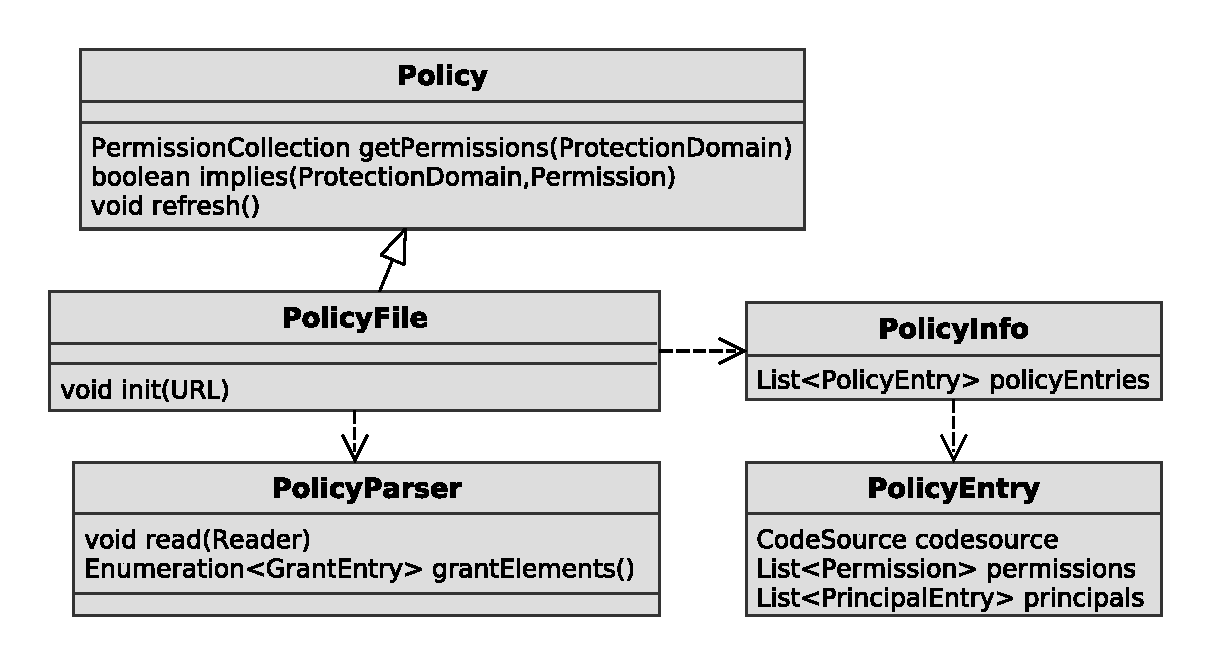
\includegraphics[width=12cm]{fig/policy-schema}
  \caption{Třídy podílející se na politice postavené na souborech politiky.}
  \label{tridyPolicyFile}
\end{figure}

Třídy podílející se na bezpečnostní politice postavené na souborech bezpečnostní politiky ukazuje diagram tříd na obrázku \ref{tridyPolicyFile}.
Tuto politiku realizuje třída {\tt PolicyFile}, podtřída třídy {\tt Policy}, která představuje obecnou bezpečnostní politiku.

Objekt politiky {\tt PolicyFile} provádí rozhodnutí o~oprávněnosti operací na základě aktuálního objektu {\tt PolicyInfo}.
Tento objekt obsahuje množinu položek bezpečnostní politiky, {\tt PolicyEntry}.

Protože tato množina je v~průběhu načítání souborů bezpečnostní politiky tvořena postupně, je umístěna v~tomto samostatném objektu.
Díky tomu je bezpečnostní politika vyměňována atomicky -- jeden objekt {\tt PolicyInfo} je v~rámci atomické reference nahrazen novým.
V~průběhu výměny bezpečnostní politiky tak nemůže dojít k~okamžiku, kdy by byla uplatňována jen z~části načtená politika.

K~inicializaci a tedy i k~načítání politiky ze souborů dochází při vytváření objektu {\tt PolicyFile} a při volání jeho metody {\tt refresh()}.
V~obou případech jsou soubory politiky určeny konfiguračními proměnnými (property) popsanými v~kapitole \ref{nastaveniPolitiky}.

%,,,,,,,,,,,,,,,,,,,,,,,,,,,,,,,,,,,,,,,,,,,,,,,,,,,,,,,,,,,,,,,,,,,,,,,,,,,,,
\subsubsection{Příklad souboru bezpečnostní politiky}
%'''''''''''''''''''''''''''''''''''''''''''''''''''''''''''''''''''''''''''''

Tento příklad ukazuje jednoduchou bezpečnostní politiku, opět v~kontextu příkladu knihovny pro přístup k~databázi z~kapitoly \ref{databazeVsouboru}.

\begin{figure}[tbh]
\begin{lstlisting}[caption=Příklad souboru bezpečnostní politiky, label=prikladSouboruBP]
grant codeBase "file:/srv/program/" {
  permission ZaznamPermission "Lucka", "nacteni";
};
grant codeBase "file:/srv/knihovna/" {
  permission ZaznamPermission "*", "nacteni";
  permission java.io.FilePermission "/srv/knihovna/data/-","read,write";
};
\end{lstlisting}
\end{figure}

Program zde má přiděleno oprávnění k~načtení záznamu \uv{Lucka}. Třída tohoto oprávnění byla definována v~kapitole \ref{zaznamPerm}.
Nemá ale přiděleno oprávnění k~přístupu k~samotným databázovým souborům.
K~těm má oprávnění přistupovat jen knihovna zpřístupňující tuto databázi, popsaná v~kapitole \ref{databazeVsouboru}.
Kvůli způsobu implementace kontroly oprávnění systémem řízení přístupu (popsaným v~kapitole \ref{implementaceAC}) je nezbytné přidělit knihovně oprávnění ke všem záznamům v~databázi, jinak by žádná kontrola oprávněnosti požadavku nemohla skončit pozitivně.

%,,,,,,,,,,,,,,,,,,,,,,,,,,,,,,,,,,,,,,,,,,,,,,,,,,,,,,,,,,,,,,,,,,,,,,,,,,,,,
\subsubsection{Zástupné znaky}
%'''''''''''''''''''''''''''''''''''''''''''''''''''''''''''''''''''''''''''''

URL kořene systému balíčků může být v~souboru bezpečnostní politiky ukončeno zástupnými znaky pomlčka ({\tt -}) a hvězdička ({\tt *}).

Zatímco {\tt /*} odpovídá všem souborům v~daném adresáři, {\tt /-} odpovídá všem souborům v~daném adresáři i jeho podadresářích, rekurzivně.
V~obou případech jsou zahrnuty jak soubory tříd ({\tt .class}), tak i celé archivy tříd ({\tt .jar}/{\tt .war}/{\tt .ear}).
Archivy vnořené v~těchto archivech však již prohledávány nejsou.
\cite{jdkdocPolicyFiles}

%-----------------------------------------------------------------------------
\subsection{Nastavení třídy a souboru bezpečnostní politiky} \label{nastaveniPolitiky}
%-----------------------------------------------------------------------------

Tato kapitola popisuje nastavení implicitní třídy a souborů bezpečnostní politiky. Změna těchto nastavení dovoluje správci počítače
stanovit bezpečnostní politiku aplikovanou implicitně na všechny programy v~Javě běžící na daném počítači.

Používaná třída a soubory bezpečnostní politiky jsou určeny globálně, pro celé běhové prostředí Javy (JRE -- Java Runtime Environment),
v~konfiguračním souboru {\tt java.security} umístěném v~podadresáři {\tt lib/security} adresáře JRE. \cite{refPolicyFiles}

Třída bezpečnostní politiky je určena svým celým jménem (např. {\tt sun.security.provider{\linebreak}.PolicyFile}) v~konfigurační proměnné {\tt policy.provider}. \cite{refPolicyFiles}

Soubory bezpečnostní politiky jsou určeny svou absolutní adresou, uvedenou včetně protokolu (pro lokální soubory {\tt file:}),
v~konfiguračních proměnných {\tt policy.url.n}, kde {\tt n} je pořadové číslo souboru. \cite{refPolicyFiles}

Načítání souborů bezpečnostní politiky začíná od {\tt policy.url.1} a postupně se {\tt n} inkrementuje a načítají se jednotlivé soubory bezpečnostní politiky,
dokud {\tt policy.url.n} existuje. \cite{refPolicyFiles}

\begin{figure}[tbh]
\begin{lstlisting}[caption=Význačnější proměnné konfiguračního souboru {\tt java.security}, label=javasecurityexample]
policy.provider=sun.security.provider.PolicyFile
policy.url.1=file:${java.home}/lib/security/java.policy
policy.url.2=file:${user.home}/.java.policy
policy.url.3=file:/my-policies/my.policy
\end{lstlisting}
\end{figure}

Příklady nastavení konfiguračních proměnných v~tomto souboru jsou uvedeny v~ukázce kódu \ref{javasecurityexample}, která je rozšířením příkladu z~knihy pana Oakse. \cite{oaks}

Nastavenou třídou bezpečnostní politiky je zde třída {\tt PolicyFile} a jako soubory bezpečnostní politiky jsou použity
soubory {\tt \$\{java.home\}/lib/security/java.policy}, {\tt \$\{user{\linebreak}.home\}/.java.policy} a {\tt /my-policies/my.policy} v~uvedeném pořadí.

Implicitně jsou používány právě první dvě uvedená umístění -- {\tt \$\{java.home\}/lib/secu{\linebreak}rity/java.policy} pro celý systém a {\tt \$\{user.home\}/.java.policy} jako jeho rozšíření pro jednotlivé uživatele. Poslední umístění je přidáno pro demonstraci, jak je možné přidat další umístění. \cite{refSecurity}

Bezpečnostní politiku je dále možné rozšířit při startu JVM o~další soubor bezpečnostní politiky. Stačí nastavit konfigurační proměnnou {\tt java.security.policy} při startu JVM: \cite{oaks}

\begin{figure}[tbh]
\begin{lstlisting}[caption=Spuštění JVM s~vlastním souborem bezpečnostní politiky, label=nastaveniBP]
java -Djava.security.policy=dalsi_soubor_politiky.policy ProgramABC
\end{lstlisting}
\end{figure}

V~tomto případě bude uvedený soubor bezpečnostní politiky použit zároveň s~výše uvedeným standardním souborem bezpečnostní politiky. Chceme-li standardní soubory bezpečnostní politiky určené souborem {\tt java.security} zcela nahradit, stačí namísto jednoho rovnítka v~definici konfigurační proměnné použít rovnítka dvě: \cite{oaks}

\begin{figure}[tbh]
\begin{lstlisting}[caption=Spuštění JVM jen s~vlastním souborem bezpečnostní politiky, label=nastaveniBP2]
java -Djava.security.policy==jediny_soubor_politiky.policy ProgramABC
\end{lstlisting}
\end{figure}

Obsah této proměnné je možné změnit i za běhu programu, má-li daná část programu oprávnění k~zápisu do této proměnné.

\begin{figure}[tbh]
\begin{lstlisting}[caption=Nastavení souboru bezpečnostní politiky zevnitř JVM, label=nastaveniBP3]
System.setProperty("java.security.policy", "jiny_soubor_politky.policy");
\end{lstlisting}
\end{figure}

Protože, jak již bylo zmíněno v~kapitole \ref{souboryBP}, nové načtení bezpečnostní politiky ze souborů bezpečnostní politiky je možné provést
skrze metodu {\tt refresh()} objektu bezpečnostní politiky, je možné provedenou změnu bezpečnostní politiky nechat projevit jejím zavoláním:

\begin{figure}[tbh]
\begin{lstlisting}[caption=Znovunačtení souboru bezpečnostní politiky, label=refreshBP]
Policy.getPolicy().refresh();
\end{lstlisting}
\end{figure}

Problémem je, že tato metoda je označena jako nedoporučovaná (deprecated), protože je implementačně závislá -- zatímco u~třídy bezpečnostní politiky {\tt PolicyFile} správně způsobí projevení změn v~souboru bezpečnostní politiky, u~jiných implementací bezpečnostní politiky může být implementována jako prázdná operace. \cite{refPolicy}

Tato práce se proto bude zabývat jen bezpečnostními politikami poskytovanými standardní implementací třídy {\tt Policy}, {\tt sun.security.provider.PolicyFile}, a na ní postavených nebo na ni delegujících implementacích.

%-----------------------------------------------------------------------------
\subsection{Statická a dynamická oprávnění ochranných domén} \label{staticPerm}
%-----------------------------------------------------------------------------

Oprávnění ochranných domén ({\tt ProtectionDomain}) popsaných v~kapitole \ref{codeSourceAprotectionDomains} jsou ukládány přímo v~objektech těchto ochranných domén,
konkrétně v~jejich atributu {\tt permissions}.~\cite{sourceProtectionDomain}

Protože jsou tato oprávnění do ochranné domény ukládány při jejím vytváření, tedy při zavádění třídy a následně nemohou být změněna, označujeme je jako statická.

Ochranné domény však souběžně mohou používat ještě oprávnění dynamická. Není-li ochranná doména označena jako používající výhradně statická oprávnění,
dotazuje se ochranná doména na oprávnění objektu bezpečnostní politiky při každém volání její metody {\tt implies()}.
Takto získaná oprávnění pak označujeme jako dynamická. \cite{sourceProtectionDomain}
Jsou-li dynamická oprávnění použita, efektivní oprávnění uplatňovaná metodou {\tt implies()} budou sjednocením dynamických a statických oprávnění třídy.
\cite{sourceProtectionDomain}

V~současnosti jsou obvykle preferována oprávnění dynamická, jež poskytují vyšší variabilitu tím, že je možné bezpečnostní politiku vyměňovat za běhu
programu -- změny v~ní se projeví jakmile začne být uplatňována metodou {\tt implies()} objektu bezpečnostní politiky, tedy zpravidla po volání metody
{\tt refresh()} používaného objektu bezpečnostní politiky.

Dynamická oprávnění jsou používána na všechny třídy zaváděné zavaděčem tříd z~URL (viz kapitola \ref{URLClassLoader}) a jsou tedy využívána ve většině programů v~Javě.
\cite{sourceURLClassLoader}

Umožňují navíc přidělovat oprávnění nejen na základě zdroje kódu, ale také na základě rolí uživatele spouštějícího daný kód. Tato dvě kritéria se však
obvykle používají pouze samostatně -- buď systém řízení přístupu ověřuje oprávnění kódu provést požadovanou operaci, nebo uživatelský kód ověřuje oprávnění
uživatele, který jej spouští, k~provedení požadované operace. V~obou případech se však stále jedná o~dynamická oprávnění.

Statická oprávnění byla v~Javě donedávna implementována jen v~zájmu zachování kompatibility s~verzemi Javy staršími než Java 2 SE 1.4. \cite{sourceProtectionDomain}
V~současnosti se však statická oprávnění opět začaly používat a to za účelem optimalizace.
Získáváním oprávnění třídy z~objektu bezpečnostní politiky pouze při zavádění třídy a ne při každém požadavku o~ověření oprávněnosti k~provedení operace je totiž možné proces ověřování oprávněnosti urychlit.

%=============================================================================
\section{Celkový pohled na bezpečnost v~Javě} \label{celkovyPohled}
%=============================================================================

\begin{figure}[ht]
  \centering
  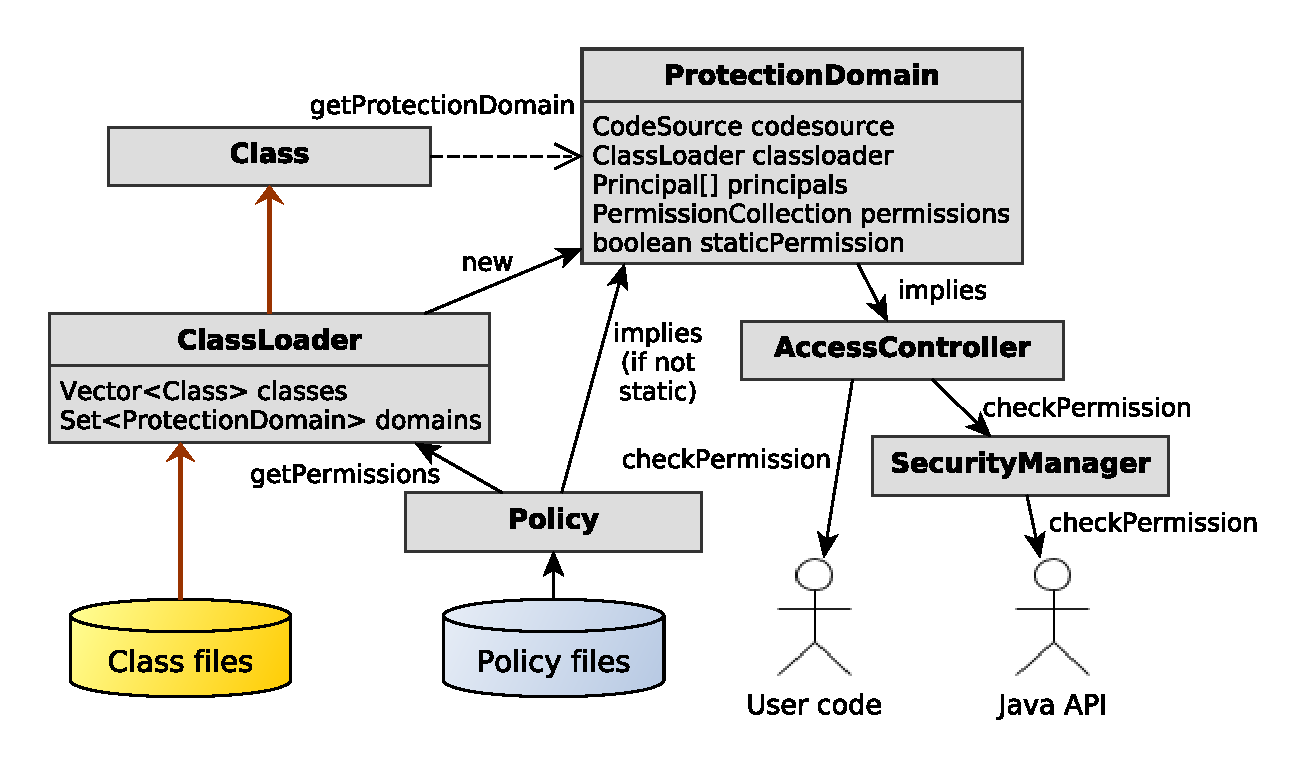
\includegraphics[width=14cm]{fig/domain-schema}
  \caption{Diagram datových toků tříd (hnědé šipky) a oprávnění tříd (černé šipky)}
  \label{diagramDatovychToku}
\end{figure}

Diagram datových toků na obrázku \ref{diagramDatovychToku} ukazuje putování informace o~oprávněních třídy ze souborů bezpečnostní politiky (Policy files) až do systému řízení přístupu ({\tt AccessController}) a správce bezpečnosti ({\tt SecurityManager}). Souvislé černé šipky představují přenos informace o~oprávněních, zatímco přerušované tlusté šipky přenos informace o~třídách. Tenké přerušované šipky představují reference. Směr šipky pak vede z~třídy objektu s~referenční proměnnou do třídy referencovaného objektu.

Ochranné domény ({\tt ProtectionDomain}) a tím i statická oprávnění třídy jsou třídám přidělovány při jejich zavádění.
Objekty ochranných domén ({\tt ProtectionDomain}) vytváří zavaděč tříd a to na základě jejich zdroje kódu ({\tt CodeSource}).
Zavaděč tříd ({\tt ClassLoader}) tak informace o~oprávněních předává objektu ochranné domény ({\tt ProtectionDomain}) při jeho vytváření.
Na statická oprávnění, která má zdroji kódu (a tedy i vytvořené ochranné doméně) zavaděč přidělit, se zavaděč dotazuje aktuálně používaného objektu bezpečnostní politiky ({\tt Policy}).

Primárním výstupem zavaděče tříd je ale objekt třídy ({\tt java.lang.Class}).
Až ten nese referenci na takto vytvořenou ochrannou doménu, kterou má společnou se všemi třídami se stejným zdrojem kódu.
Zavádění tříd podrobněji viz kapitola \ref{classloader}.

Systém řízení přístupu ({\tt java.security.AccessController}) pak při dotazu {\tt checkPermission()} ze strany uživatele nebo ze strany správce bezpečnosti rozhoduje o~povolení operace na základě odpovědí na jeho dotaz {\tt implies()} položený ochranným doménám tříd na zásobníku volání.
Informace o~oprávněních tak putují z~objektu ochranné domény do systému řízení přístupu, jak je znázorněno na obrázku.

Metoda {\tt implies()} ochranné domény ({\tt ProtectionDomain}) rozhoduje v~závislosti na tom, zda je nastavena jako používající výhradně statická oprávnění.
Pokud ano, rozhoduje jen na základě statických oprávnění uložených do ochranné domény při jejím vytváření.
V~opačném případě se zároveň dotazuje také objektu bezpečnostní politiky ({\tt Policy}).
Cesta informace o~oprávněních z~objektu bezpečnostních politiky do ochranné domény je také znázorněna na obrázku.

Na systém řízení přístupu pak dotaz {\tt checkPermission()} deleguje také standardní správce bezpečnosti ({\tt java.lang.SecurityManager}), což je znázorněno na obrázku jako putování informace ze systému řízení přístupu do objektu správce bezpečnosti.


%%%%%%%%%%%%%%%%%%%%%%%%%%%%%%%%%%%%%%%%%%%%%%%%%%%%%%%%%%%%%%%%%%%%%%%%%%%%%%
\chapter{Distribuované prostředí Red Hat JBoss} \label{jboss}
%%%%%%%%%%%%%%%%%%%%%%%%%%%%%%%%%%%%%%%%%%%%%%%%%%%%%%%%%%%%%%%%%%%%%%%%%%%%%%

Tato kapitola popisuje prostředí aplikačního serveru WildFly, dříve známého jako JBoss Application Server.
Podrobněji pak rozebírá možnosti používání bezpečnostních politik Javy v~prostředí tohoto aplikačního serveru.

%=============================================================================
\section{Úvod do WildFly (JBoss AS)} \label{uvodWildFly}
%=============================================================================

WildFly, dříve známý jako JBoss Application Server, je aplikační server standardu Java EE (Enterprise Edition).
Poskytuje běhové prostředí (nejen) Java EE aplikacím, které jsou na tomto aplikačním serveru nainstalovány.
\cite{wildflyRename}

Jednotlivé instalace WildFly nazýváme hostiteli (host). Hostitel typicky odpovídá jednomu fyzickému serveru.
V~rámci každého hostitele může běžet více serverů (server).
Hostitelé mohou být spojováni do domén (domain), přičemž jeden z~nich v~takovém případě zastává roli tzv. doménového řadiče (domain controller).
Ostatní hostitelé domény se k~němu pak registrují a je na ně aplikována doménová konfigurace.
\cite{jbossDomainSetup}

Doménová konfigurace je uložena v~konfigurační souboru domény, {\tt domain.xml}, uložené právě na doménovém řadiči.
Tento soubor obsahuje konfiguraci skupin serverů a profilů serverů.
Konfigurace profilů pak zahrnuje také konfiguraci subsystémů používaných na serverech domény používajících daný profil.
\cite{jbossDomainSetup}

Každý hostitel má zároveň vlastní konfigurační soubor {\tt host.xml}.
Tento soubor určuje název hostitele, zda-li je tento hostitel doménovým řadičem a, pokud není, také adresu doménového řadiče.
Zde jsou definovány servery, které na daném hostiteli poběží, porty, na kterých budou poskytovat své služby, a skupiny, do kterých budou patřit.
\cite{jbossDomainSetup}

Distribuovanosti prostředí je docíleno nasazováním aplikací (deployment) na celé skupiny serverů najednou.
Požadavky směřované na aplikace pak jsou rozprostírány mezi všechny servery domény osazené danou aplikací pomocí tzv. vyvažovačů zátěže (load balancer).
\cite{jbossLoadBalancing}

Vyvažovač zátěže umožňuje skrýt celou doménu serverů za jedinou IP adresu.
Na této adrese pak naslouchá požadavkům a předává je jednotlivým serverům této domény -- zpravidla tomu, který je v~daný okamžik nejméně vytížený.
\cite{jbossLoadBalancing}

%=============================================================================
\section{Rozhraní pro správu WildFly} \label{managementAPI}
%=============================================================================

Tato podkapitola popisuje rozhraní umožňující správu aplikačních serverů WildFly, {\bf JBoss management API}.
Toto rozhraní umožňuje spravovat doménu WildFly a provádět změny v~konfiguraci domény i jednotlivých serverů.
\cite{jbossDetypedManagement}

Rozhraní zpřístupňuje konfiguraci ve formě stromové struktury, skládající se z~konfiguračních uzlů a konfiguračních vlastností.
Zatímco konfigurační uzly se mohou libovolně zanořovat, vlastnosti mohou být jen listy této stromové struktury.
\cite{jbossDetypedManagement}

Pro reprezentaci dotazů nad touto stromovou strukturou i odpovídajících odpovědí je využívána dynamická reprezentace modelu (DMR -- Dynamic Model Representation).
DMR všechny informace (např. dotaz nebo odpověď Management API) ukládá jako strom uzlů -- objektů třídy {\tt ModelNode}.
\cite{jbossDetypedManagement}

Na rozdíl od uzlů konfiguračního stromu může být obsahem uzlu {\tt ModelNode} hodnota jednoho z~definovaných datových typů (viz \cite{jboss7slideShare}) nebo seznam jiných uzlů. Ne však obojí zároveň.
\cite{jboss7slideShare}

Klienti JBoss Management API mohou aplikačnímu serveru pokládat dotazy ve formě uzlů DMR a žádat tak o~provedení operace nad konfiguračním stromem.
Výsledek této operace je pak opět ve formě uzlu DMR předán dotazujícímu se klientovi.
\cite{jbossDetypedManagement}

Operace mohou sloužit jak ke čtení dat z~konfiguračního stromu a k~jejich zápisu, tak i k~provádějí jiných akcí souvisejících se správou serverů nebo domény.
Příklady posledního uvedeného typu operace mohou být operace startu ({\tt start}) nebo znovunačtení ({\tt reload}) serveru.
Každý uzel konfiguračního stromu může mít jinou množinu operací, které nad ním lze provádět.
Na tuto množinu operací je možné se serveru dotázat.
\cite{jbossDetypedManagement}

%-----------------------------------------------------------------------------
\subsection{Rozšíření WildFly} \label{rozsireniWildFly}
%-----------------------------------------------------------------------------

Funkce poskytované aplikačním serverem aplikacím i jeho správcům je možné různými způsoby rozšiřovat za pomoci rozšíření.
Typickým obsahem rozšíření je subsystém. Subsystémy jsou konfigurovány pro jednotlivé konfigurační profily, tedy pro všechny servery používající daný profil.

Pro potřeby této práce důležité zmínit hlavně to, že rozšíření může vytvářet vlastní typy uzlů konfiguračního stromu.
Těmto uzlům může definovat vlastnosti, které mohou mít.
Uzlům i vlastnostem pak mohou přidělovat třídy ošetřující operace nad nimi.
\cite{WildFlyExtending}

Je tak například možné definovat typ uzlu, který při svém vytvoření nebo smazání spustí speciální metodu pro tento účel vytvořeného objektu.
Metody podobných objektů mohou být spouštěny také při nastavení hodnoty nebo nastavení nedefinované hodnoty konfigurační vlastnosti tohoto uzlu.

V~podstatě nic co běží v~rámci WildFly, ať již součásti WildFly nebo uživatelské aplikace, neběží celou dobu běhu aplikačního serveru.
Pouze si zaregistrují události, na které později, až se vyskytnou, reagují -- říkáme že vše co běží v~rámci WildFly je služba. \cite{jboss7slideShare}

Běžnějším příkladem registrované události, než jakou je úprava konfiguračního uzlu, je příchod HTTP požadavku se specifikovanou URL.
Takové události jsou typicky registrovány Servlety v~rámci své definice v~konfiguračním souboru {\tt web.xml} své aplikace.
\cite{jboss7slideShare}

%-----------------------------------------------------------------------------
\subsection{Webová konzola WildFly} \label{hal}
%-----------------------------------------------------------------------------

Webová konzola WildFly je standardní součástí aplikačního serveru WildFly.
Je GWT (Google Web Toolkit) aplikací běžící na straně klienta, ve webovém prohlížeči.
Aplikační server tato aplikace spravuje prostřednictvím JBoss Management API.
Konkrétně využívá jeho variantu běžící nad protokolem HTTP, která dotazy na API zasílá ve formě HTTP POST požadavků, jejichž tělem je JSON reprezentace uzlu DMR, {\tt ModelNode}. Obdobným způsobem pak server zasílá odpověď.
\cite{WildFlyManagementAPIreference}

%=============================================================================
\section{Běh WildFly se správcem bezpečnosti} \label{wildflySeSM}
%=============================================================================

Tato podkapitola se zabývá problémem používání správce bezpečnosti a bezpečnostních politik v~prostředí JBoss/WildFly.

Na první pohled se může zdát, že nakonfigurovat použití správce bezpečnosti na aplikační server WildFly je možné stejně jako na jakoukoli jinou aplikaci v~Javě -- nastavením patřičných konfiguračních vlastností (popsaných v~kapitolách \ref{securityManager} a \ref{nastaveniPolitiky}) při startu JVM za pomoci k~tomu určeného parametru {\tt -D} příkazu {\tt java}.

Ve spouštěcím skriptu WildFly ({\tt standalone.sh} / {\tt domain.sh} / {\tt standalone.bat} / {\tt domain.bat}) je pro potřeby přidávání vlastních parametrů příkazu {\tt java} používána proměnná {\tt JAVA\_OPTS}.
Připojením potřebných parametrů na konec hodnoty této proměnné bychom tedy měli dosáhnout použití správce bezpečnosti a stanovené bezpečnostní politiky ve všech JVM aplikačního serveru.
Kód který by k~tomu do spouštěcího skriptu musel být přidán ukazuje (pro {\tt *.sh} variantu) ukázka kódu \ref{wildflySeSMcode}.
Každý její řádek přidá na konec proměnné {\tt \$JAVA\_OPTS} jeden parametr příkazu {\tt java} potřebný ke spouštění serveru s~bezpečnostní politikou.
\cite{jbossSecurityManager}

\begin{figure}[tbh]
\begin{lstlisting}[caption=Doplnění spouštěcího skriptu o~použití správce bezpečnosti, label=wildflySeSMcode]
JAVA_OPTS="$JAVA_OPTS -Djava.security.manager"
JAVA_OPTS="$JAVA_OPTS -Djava.security.policy==wildfly.policy"
\end{lstlisting}
\end{figure}

Uvedený soubor bezpečnostní politiky ({\tt wildfly.policy}) prozatím ponecháme prázdný.
Zkusíme-li nyní aplikační server spustit, spuštění skončí neúspěchem kvůli chybějícím oprávněním, nezbytných k~běhu aplikačního serveru. Tento výsledek je ale pro nás pozitivní, neboť prokazuje, že aplikační server byl bezpečnostní politikou skutečně omezen.

Do souboru bezpečnostní politiky dále přidáme přidělení všech oprávnění veškerému kódu běžícímu v~rámci aplikačního serveru. Vzniklý soubor bezpečnostní politiky ukazuje ukázka kódu \ref{wildflyPolicy}.

\begin{figure}[tbh]
\begin{lstlisting}[caption=První testovací soubor bezpečnostní politiky, label=wildflyPolicy]
grant {
    permission java.security.AllPermission;
};
\end{lstlisting}
\end{figure}

Zopakujeme-li experiment, zjistíme že s~takto nastavenou bezpečnostní politikou se aplikační server bez problémů spustil a bez problému funguje.
Podrobnějším zkoumáním však zjistíme, že na uživatelské aplikace se tato benevolentní bezpečnostní politika neuplatňuje.
Zatímco zapnutí správce bezpečnosti tedy možnosti uživatelských aplikací skutečně omezilo, nastavení vše povolujících bezpečnostních politik uživatelským
aplikacím žádné z~odebraných schopností nenavrátilo.

%-----------------------------------------------------------------------------
\subsection{Zavaděč tříd modulů WildFly} \label{moduleClassLoader}
%-----------------------------------------------------------------------------

Tato podkapitola popisuje jádro problému s~bezpečnostními politikami ve WildFly -- zavaděč tříd modulů WildFly ({\tt org.jboss.modules.ModuleClassLoader}).

Zavaděč tříd se podařilo jako viníka odhalit postupným krokováním programu.
To potvrdilo, že objekty bezpečnostní politiky produkují správná oprávnění.
Zároveň ale ukázalo, že do ochranných domén tříd jsou ukládány oprávnění jiná.
Jak vyplývá z~popisu cesty oprávnění ze souborů bezpečnostních politik do ochranných domén v~kapitole \ref{celkovyPohled},
jediným mezičlánkem, který tedy mohl s~oprávněními v~této době manipulovat, je právě zavaděč tříd.

Tento předpoklad pohled do zdrojového kódu zavaděče tříd modulů potvrdil -- tento zavaděč oprávnění poskytovaná objektem bezpečnostní politiky implicitně ignoruje.
Namísto toho třídám do ochranných domén ukládá oprávnění určená specifikací Java EE. \cite{javaEEspec}
(Ta jsou v~případě uživatelských aplikací upravitelná souborem {\tt permission.xml}.)

Zároveň však byla nalezena konfigurační proměnná (property), která toto chování umož-{\linebreak}ňuje změnit.
Bude-li konfigurační proměnná {\tt jboss.modules.policy-permissions} nastavena na hodnotu {\tt true}, bude zavaděč tříd modulů do ochranných domén ukládat jak oprávnění určená specifikací Java EE, tak i oprávnění z~objektů bezpečnostní politiky.
Množina efektivních oprávnění třídy pak bude odpovídat sjednocení těchto dvou množin oprávnění.
\cite{sourceModuleClassLoader}

Ukázka kódu \ref{jbossOpts} ukazuje všechny definice konfiguračních proměnných, které musí být do spouštěcího skriptu aplikačního serveru WildFly přidány,
aby byl server a aplikace které v~něm běží omezeny oprávněními stanovenými uvedeným souborem bezpečnostní politiky (v~příkladu {\tt directory/wildfly.policy}).

\begin{figure}[tbh]
\begin{lstlisting}[caption=Úprava spouštěcího skriptu pro spuštění s~bezpečnostní politikou, label=jbossOpts]
JAVA_OPTS="$JAVA_OPTS -Djboss.modules.policy-permissions=true"
JAVA_OPTS="$JAVA_OPTS -Djava.security.manager"
JAVA_OPTS="$JAVA_OPTS -Djava.security.policy==directory/wildfly.policy"
\end{lstlisting}
\end{figure}

%-----------------------------------------------------------------------------
\subsection{Úpravy zavaděče tříd modulů WildFly} \label{upravaZavadeceWildFly}
%-----------------------------------------------------------------------------

Tato podkapitola popisuje úpravy zavaděče tříd modulů WildFly, které bylo nutné provést, aby bylo možné vyměňovat bezpečnostní politiky za běhu aplikačního serveru.

Jakékoli snahy o~výměnu bezpečnostní politiky za běhu aplikačního serveru se doposud jevily jako marné. Oprávnění totiž byly nastavována jako statická.
Jsou tedy z~objektu bezpečnostní politiky načítána pouze při načítání třídy. Změny bezpečnostní politiky se tak projevovaly pouze na nově načítaných třídách.

Protože je cílem výměna bezpečnostní politiky za běhu aplikačního serveru, je tento stav nedostačující.
Aby byla možná změna bezpečnostní politiky za běhu aplikačního serveru, je nezbytné, aby byla oprávnění používána jako dynamická, jak je popsáno v~kapitole \ref{staticPerm}.
V~rámci této práce byla tedy vytvořena záplata zavaděče tříd modulů WildFly, která umožňuje používání dynamických oprávnění ve WildFly.

\begin{figure}[b!]
\begin{lstlisting}[caption=Hlavní část záplaty umožňující nastavit používání dynamických oprávnění, label=refreshable]
+  if (POLICY_REFRESHABLE) {
+      protectionDomain = new ProtectionDomain(codeSource, permissions,
+                                 this, null); // staticPermission=false
+  } else if (POLICY_PERMISSIONS && POLICY_READY.get()) {
-  if (POLICY_PERMISSIONS && POLICY_READY.get()) {
\end{lstlisting}
\end{figure}

Zatímco řešení popsané v~předchozí kapitole ukládalo do ochranných domén množinu oprávnění,
která byla sjednocením oprávnění udělených dle specifikace Java EE a oprávnění z~objektu bezpečnostní politiky,
v~této variantě jsou do ochranné domény ukládány opět jen oprávnění udělená dle specifikace Java EE.
Při vytváření této ochranné domény je ale použit konstruktor se všemi čtyřmi parametry, čímž je tato doména označena jako používající dynamická oprávnění.
Při každém dotazu na oprávnění k~provedení potenciálně nežádoucí operace tak je tento dotaz předán objektu bezpečnostní politiky.
Efektivní oprávnění třídy pak jsou sjednocením dynamických oprávnění z~objektu bezpečnostní politiky a statických oprávnění přidělených dle specifikace Java EE při načítání třídy.

Použití této nové varianty bylo přitom záměrně omezeno, aby bylo možné začlenění této úpravy do vývojové větve WildFly.
Byla vytvořena nová konfigurační vlastnost {\tt jboss.modul es.policy-refreshable}, jejíž hodnota určuje, zda-li mají být dynamická oprávnění použita.
Je-li její hodnota {\tt true}, budou použita dynamická oprávnění, jinak budou používána statická oprávnění jako doposud.
O~začlenění této záplaty do vývojové větve bylo požádáno \cite{jmPullRequest}.

%-----------------------------------------------------------------------------
\subsection{Výměna bezpečnostní politiky za běhu} \label{zmenaZaBehu}
%-----------------------------------------------------------------------------

Tato podkapitola popisuje postup, který je nutné použít, aby bylo možné z~aplikace nebo z~rozšíření WildFly provést výměnu bezpečnostní politiky.

Jak již bylo popsáno v~kapitole \ref{nastaveniPolitiky}, pro výměnu bezpečnostní politiky je nutné pozměnit hodnotu konfigurační proměnné
{\tt java.security.policy} a vyžádat od objektu bezpečnostní politiky znovunačtení souboru bezpečnostní politiky.
V~prostředí WildFly však, přestože již je zajištěno používání dynamických oprávnění (viz kapitola \ref{upravaZavadeceWildFly}), bohužel nestačí zavolat metodu {\tt refresh()} aktuálně používaného objektu bezpečnostní politiky. Tímto objektem je totiž instance třídy {org.jboss.security.jacc.DelegatingPolicy}. Tento objekt sice všechny volání metody {\tt implies()} nesouvisející s~JACC (Java Authorization Contract for Containers) deleguje na původní objekt bezpečnostní politiky, metodu {\tt refresh()} na něj však nedeleguje.

Toto chování jsem nahlásil jako chybu implementace třídy {\tt DelegatingPolicy}, neboť jsem přesvědčen, že takové počínání je nelogické. Deleguje-li třída dotazování, měla by delegovat také žádost o~znovunačtení dat, na základě kterých jsou tato rozhodnutí prováděna. \cite{issueDelegating}

\begin{figure}[tbh]
\begin{lstlisting}[caption=Znovunačtení bezpečnostní politiky při nastavené {\tt DelegatingPolicy}, label=refreshDelegating]
    Class<?> delegatingPolicy = Class.forName("org.jboss.security.jacc.DelegatingPolicy");
    Field f = delegatingPolicy.getDeclaredField("delegate");
    f.setAccessible(true);
    Policy in = (Policy) f.get(Policy.getPolicy());
    in.refresh();
\end{lstlisting}
\end{figure}

Pro potřeby této bakalářské práce však bylo znovunačtení bezpečnostní politiky prozatím zajištěno za pomoci reflexe, jak je ukázáno v~ukázce kódu \ref{refreshDelegating}.
Reflexí je zde získána hodnota atributu {\tt delegate} aktuálně používaného objektu bezpečnostní politiky, který je třídy {\tt DelegatingPolicy}.
Hodnotou {\tt delegate} je další objekt bezpečnostní politiky, zavolání jehož metody {\tt refresh()} již postačuje k~dosažení znovunačtení bezpečnostní politiky ve WildFly.

%%%%%%%%%%%%%%%%%%%%%%%%%%%%%%%%%%%%%%%%%%%%%%%%%%%%%%%%%%%%%%%%%%%%%%%%%%%%%%
\chapter{Návrh systému} \label{navrh}
%%%%%%%%%%%%%%%%%%%%%%%%%%%%%%%%%%%%%%%%%%%%%%%%%%%%%%%%%%%%%%%%%%%%%%%%%%%%%%

V~této kapitole je navržen způsob implementace systému pro centralizovanou správu a distribuci bezpečnostních politik.

%=============================================================================
\section{Specifikace problému} \label{specifikaceProblemu}
%=============================================================================

Tato práce řeší problém, jakým způsobem používat bezpečnostní politiky Javy v~distribuovaných prostředích aplikačních serverů WildFly.
Tato prostředí jsou typicky tvořena skupinou několika (nebo i mnoha) aplikační serverů seskupených do domény WildFly.

Pravděpodobně nejjednodušším možným řešením, jak bezpečnostní politiky na tyto domény serverů nasazovat, je použít stejné řešení, jaké bylo v~kapitole \ref{wildflySeSM} použito pro nasazení politiky na samostatný server.

Tento způsob je ale poměrně pracný, neboť pro každou změnu bezpečnostní politiky vyžaduje zkopírování tohoto souboru na jednotlivé servery nebo úpravu jeho adresy ve spouštěcího skriptu WildFly. Následně je navíc nutné server WildFly restartovat.

Cílem této práce proto je, implementovat řešení pro správu bezpečnostních politik, splňující následující požadavky:

\begin{itemize}
  \item Mělo by umožnit nastavovat použití bezpečnostní politiky na serverech domény.
%  \item Mělo by umožňovat provádět toto nastavení {\bf hromadně} -- pro celé skupiny serverů domény najednou. % toto je na urovni GUI
  \item Mělo by umožňovat provádět toto nastavení {\bf centrálně} -- z~jediného místa.
  \item Nemělo by vyžadovat ruční {\bf přenos souborů} bezpečnostní politiky mezi servery, na kterých mají být použity.
  \item Nemělo by vyžadovat {\bf restart} serverů domény pro projevení změn v~nastavení politiky.
\end{itemize}

Návrhy řešení uvedených požadavků zpracovávají následující kapitoly.

%=============================================================================
\section{Možnosti řešení} \label{vycetMoznostiReseni}
%=============================================================================

Možnosti řešení problému popsaného v~kapitole \ref{specifikaceProblemu} jsou následující:

\begin{itemize}
  \item Používat jako soubor bezpečnostní politiky soubor uložený v~jednom společném umístění.
  \item Zajistit přenos souborů bezpečnostní politiky samostatným programem nebo rozšířením WildFly.
\end{itemize}

Všechny varianty jsou podrobněji popsány v~následujících podkapitolách.

%-----------------------------------------------------------------------------
\subsection{Společné umístění souboru bezpečnostní politiky} \label{reseniSpolecne}
%-----------------------------------------------------------------------------

Poměrně jednoduchým řešením problému by mohlo být nastavit na serverech domény ručně soubor bezpečnostní politiky, ležící v~umístění společném pro všechny servery domény.
Pro jakoukoli změnu bezpečnostní politiky by pak stačilo upravit tento jeden společný soubor bezpečnostní politiky.

Sdíleným umístěním by mohl být adresář sdílený například prostřednictvím protokolu FTP (File Transfer Protocol), NFS (Network File System) nebo HTTP (Hypertext Transfer Protocol).
Toto umístění by bylo příhodné umístit na doménový řadič, který zajišťuje šíření i ostatní konfigurace mezi servery domény.

Ačkoli toto řešení poměrně elegantně řeší problém změny obsahu souboru bezpečnostní politiky, problematičtější už je používání více souborů bezpečnostní politiky na různých serverech a přepínání mezi nimi.
Tento problém je možné vyřešit za pomoci symbolických odkazů -- soubor používaný JVM by byl symbolickým odkazem daného serveru.
Namísto výměny adresy souboru bezpečnostní politiky na straně serveru by tak byl vyměňován cíl odkazu tohoto symbolického odkazu.

Problémem, který přetrvává, je ale způsob, jak zajistit znovunačtení souboru bezpečnostní politiky, a zajistit tak nové načtení bezpečnostní politiky.
To může zajistit jen aplikace běžící v~rámci JVM jednotlivých serverů nebo restart celého aplikačního serveru.

Chceme-li tedy zajistit výměnu bezpečnostní politiky bez potřeby restartu aplikačního serveru, je možné vytvořit program,
který bude nasazen na všech serverech domény a bude naslouchat požadavkům na znovunačtení bezpečnostní politiky.
Tento program je možné implementovat ve formě Java EE aplikace nebo ve formě rozšíření aplikačního serveru WildFly.
V~tomto případě však ke druhé, složitější, variantě není žádný racionální důvod.

%-----------------------------------------------------------------------------
\subsection{Přenos souborů bezpečnostní politiky samostatným programem} \label{reseniProgramem}
%-----------------------------------------------------------------------------

V~předchozí variantě byl program nasazený na serverech domény využíván jen ke znovunačítání bezpečnostní politiky.
Tato varianta počítá s~jeho využitím také k~nastavení a přenosu samotného souboru bezpečnostní politiky.
Soubor bezpečnostní politiky by přitom stačilo na server, na který má být nasazen, uložit až těsně před tím, než by měl být nastaven.
K~jeho uložení by přitom postačoval dočasný soubor, který by následně, po vyvolání znovunačtení bezpečnostní politiky, mohl být bezpečně smazán.
Soubor bezpečnostní politiky totiž musí na serveru existovat jen po, kdy je jeho obsah načítán,
k~čemuž v~tomto případě bude probíhat jen v~souvislosti se znovunačítáním bezpečnostní politiky.

Byla by-li tato aplikace implementována jako rozšíření aplikačního serveru WildFly, jakým je například subsystém,
mohla by k~ukládání a distribuci souborů bezpečnostních politik využívat konfigurační strom WildFly.
Nebylo by tak třeba žádného speciálního úložiště souborů bezpečnostní politiky -- soubory bezpečnostní politiky
by tak byly uloženy společně s~konfigurací většiny součástí WildFly v~konfiguračním souboru domény.
(O~konfiguračních souborech WildFly více v~kapitole \ref{uvodWildFly}.)

Tím, že by soubory bezpečnostní politiky byly uloženy v~konfiguračním stromě WildFly by navíc bylo možné provádět znovunačítání
bezpečnostní politiky v~reakci na událost změny používané bezpečnostní politiky.
Na změnu hodnoty v~konfiguračním stromu WildFly je totiž při její definici možné provést navázání akce. (viz kapitola \ref{rozsireniWildFly})

%=============================================================================
\section{Výběr řešení} \label{vyberReseni}
%=============================================================================

Jako lepší řešení bylo zvoleno druhé uvedené řešení -- řešení ve formě programu provádějícího jak znovunačítání, tak také distribuci souborů bezpečnostní politiky.
Zvoleno bylo kvůli menším nárokům na instalaci a správu takového řešení -- zatímco první řešení by vyžadovalo jak přípravu sdíleného umístění souborů politiky, tak i instalaci programu umožňujícího provést znovunačtení politiky, zvolené řešení vystačí jen s~instalací implementovaného programu.
Případné nižší nároky na implementaci tohoto programu nemohou v~tomto případě omluvit vyšší nároky na správu výsledného řešení.

Jako vhodný způsob implementace tohoto programu, zajišťujícího distribuci a znovunačítání souborů bezpečnostní politiky byla dále zvolena varianta ve formě rozšíření aplikačního serveru WildFly.
Výhody spojené s~využíváním konfiguračního stromu WildFly pro ukládání souborů bezpečnostní politiky převyšují zvýšené nároky na implementaci programu ve formě rozšíření WildFly, namísto implementace ve formě Java EE aplikace.

%=============================================================================
\section{Návrh uživatelského rozhraní} \label{navrhGUI}
%=============================================================================

Součástí zadání práce bylo také vytvoření webového rozhraní pro komunikaci implementovaného systému s~uživatelem.
Toto webové rozhraní by tedy mělo umožňovat následující:

\begin{itemize}
  \item Zobrazovat bezpečnostní politiku nasazenou na zvoleném serveru domény.
  \item Upravovat soubory bezpečnostní politiky uložené v~konfiguračním stromu WildFly.
  \item Nasazovat tyto soubory bezpečnostní politiky na jednotlivé servery domény.
  \item Nasazovat tyto soubory bezpečnostní politiky na celé skupiny serverů domény.
  \item Vypínat používání bezpečnostní politiky na serverech nebo jejich skupinách.
\end{itemize}

Jelikož je samotné jádro řešení implementováno jako subsystém WildFly, jako logické řešení se nabízí implementovat uživatelské rozhraní tohoto subsystému jako rozšíření webové konzoly WildFly.
Toto rozhraní bylo navrženo jako tři nové konfigurační obrazovky webové konzoly WildFly:

\begin{enumerate}
  \item Obrazovka {\bf Servers} (Servery) umožňuje zvolit, které bezpečnostní politiky mají být nasazeny na jednotlivých serverech a skupinách domény. Nastavením prázdné (None/{\tt null}) bezpečnostní politiky navíc umožňuje používání bezpečnostní politiky na serveru nebo skupině vypnout.
  \item Obrazovka {\bf Policies} (Politiky) umožňuje vytvářet, upravovat a odstraňovat samotné bezpečnostní politiky. Ty pak mohou být jednotlivým serverům přidělovány na obrazovce {\bf Servers}.
  \item Obrazovka {\bf JSM Policy} (Politika správce bezpečnosti Javy) umožňuje zobrazit bezpečnostní politiku nasazenou na vybraném serveru -- její název a obsah.
\end{enumerate}

\begin{figure}[ht]
  \centering
  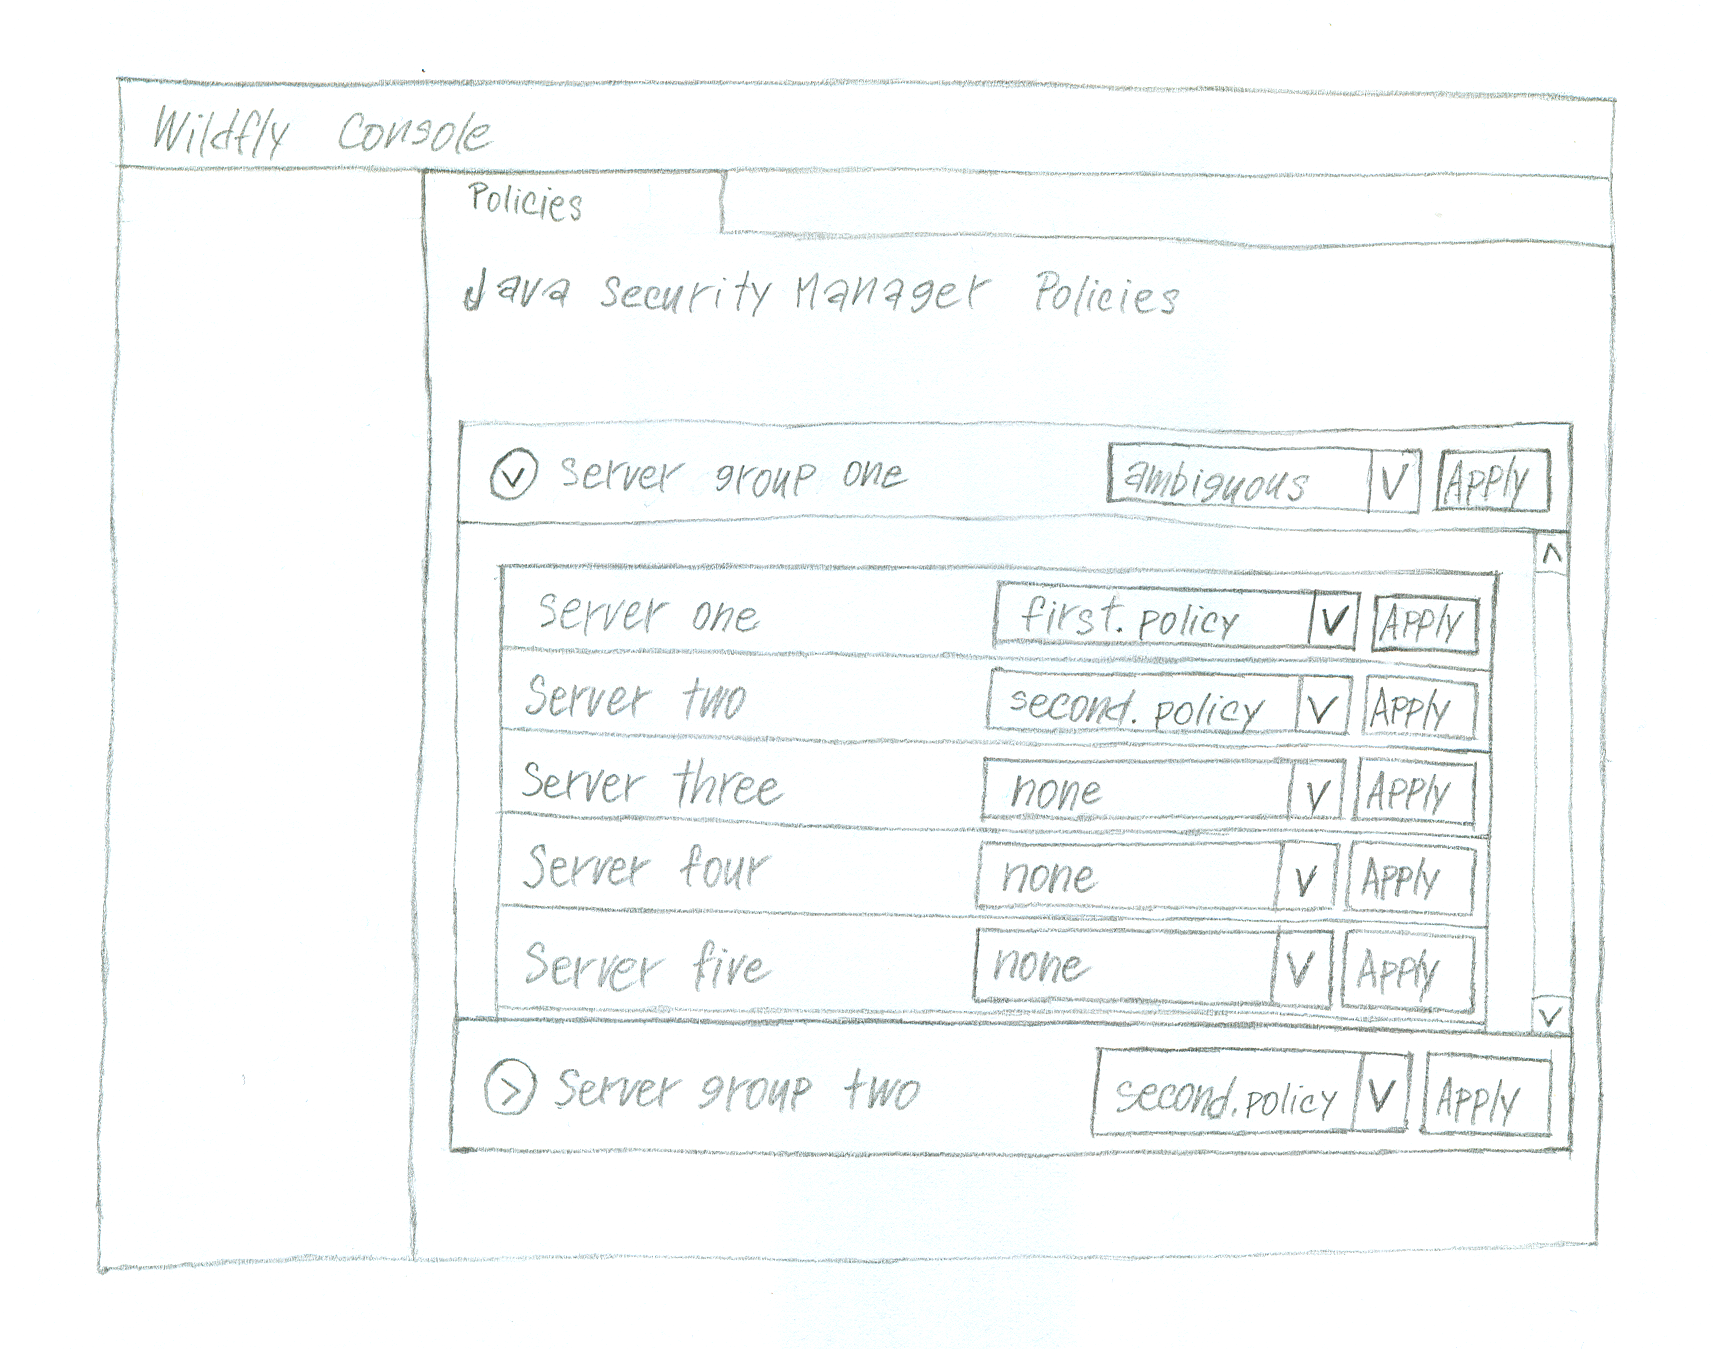
\includegraphics[width=14cm]{fig/mockup}
  \caption{Grafický návrh uživatelského rozhraní plánovaného rozšíření WildFly.}
  \label{navrhGui}
\end{figure}

\begin{figure}[ht]
  \centering
  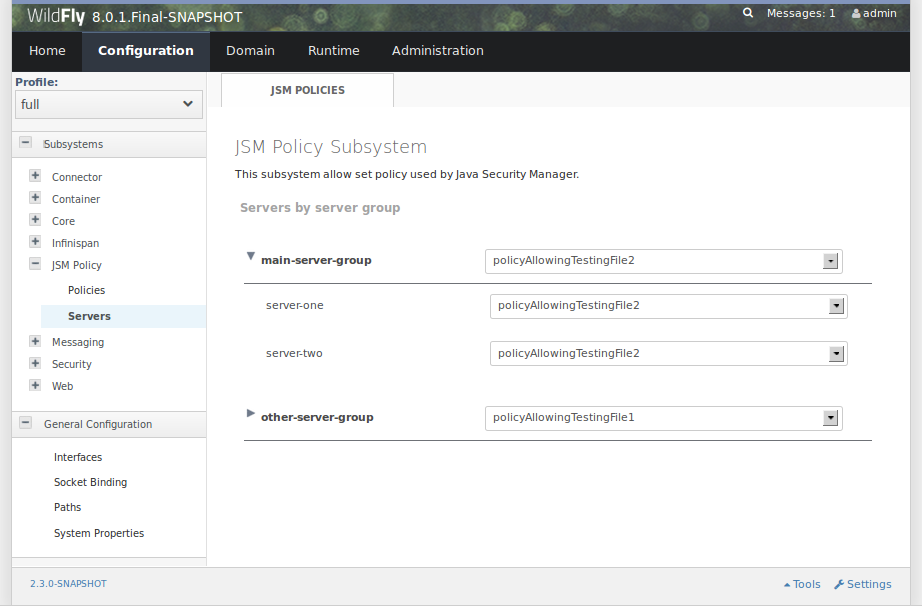
\includegraphics[width=14cm]{fig/jsmpolicy-servers}
  \caption{Výsledná podoba webového uživatelského rozhraní.}
  \label{vysledneGui}
\end{figure}

Grafický návrh první uvedené konfigurační obrazovky, umožňující zvolit, které bezpečnostní politiky mají být nasazeny na jednotlivých serverech a skupinách, je vyobrazen na obrázku \ref{navrhGui}. Zároveň je pro srovnání na obrázku \ref{vysledneGui} ukázán snímek obrazovky ukazující výslednou podobu této konfigurační obrazovky, jak byla později implementována.

Jako způsob výběru bezpečnostní politiky serveru i skupiny byla zvolena omezená nabídka. Tato nabídka umožňuje výběr jedné bezpečnostní politiky ze seznamu politik vytvořených prostřednictvím druhé konfigurační obrazovky. Umožňuje zároveň vypnout používání bezpečnostní politiky výběrem speciální hodnoty {\bf none} (žádná). Další speciální hodnota {\bf ambiguous} (neurčitá) má signalizovat, že servery skupiny používají různé bezpečnostní politiky.

Celou konfigurační obrazovku mimo nadpisu tvoří seznam skupin v~doméně. Každou položku tohoto seznamu přitom tvoří tlačítko pro zobrazení seznamu serverů obsažených v~této skupině, název skupiny, výše popsaná nabídka pro výběr politiky pro celou skupinu najednou a tlačítko pro uložení změny výběru.

Použitím tlačítka pro zobrazení seznamu serverů skupiny je pod položkou skupiny zobrazen server serverů této skupiny podobný seznamu serverů. Jeho položky jsou tvořeny názvem serveru, nabídkou pro výběr politiky a tlačítkem pro uložení změny.

Na obrázku \ref{vysledneGui} je navíc vidět také základní ovládací prvky webové konzoly WildFly, které jsou v~návrhu vyobrazeny jen schématicky.
V~levé části obrazovky se nachází menu subsystémů -- umožňuje navigaci mezi konfiguračními obrazovkami jednotlivých subsystémů WildFly ve zvoleném profilu.
Vrchní menu zobrazuje informace o~systému, přihlášeném uživateli a umožňuje navigovat mezi jednotlivými části WildFly konzoly.

Odkaz na konfigurační obrazovky {\bf Servers} a {\bf Policies} se nachází v~části {\bf Configuration} (Konfigurace), je-li přepnuta na profil, v~kterém je nainstalován implementovaný subsystém. Konfigurační obrazovka {\bf JSM Policy} zobrazující informace o~politice nasazené na zvoleném serveru je v~části {\bf Runtime} (Za běhu).

Webová konzola umožňuje také rozdělit jednu konfigurační obrazovku na více panelů. (Příklad panelu je na obrázku \ref{navrhGui} popsán jako {\bf Policies}.)
Této možnosti však v~tomto rozšíření webové konzoly není využito.

%%%%%%%%%%%%%%%%%%%%%%%%%%%%%%%%%%%%%%%%%%%%%%%%%%%%%%%%%%%%%%%%%%%%%%%%%%%%%%
\chapter{Popis implementace systému} \label{implementace}
%%%%%%%%%%%%%%%%%%%%%%%%%%%%%%%%%%%%%%%%%%%%%%%%%%%%%%%%%%%%%%%%%%%%%%%%%%%%%%

Implementace řešení byla rozdělena do několika etap. V~první etapě byl vytvořen první prototyp systému umožňující nasazení bezpečnostní politiky na základě hodnoty konfigurační vlastnosti, v~které byla prozatím jen URL adresa tohoto souboru. Tento prototyp prokázal, že nasazování bezpečnostních politik implementovaným způsobem je možné.

Teprve následně byla implementována konečná verze řešení, jež do konfiguračního stromu WildFly ukládala soubory politik ve formě konfiguračních uzlů a uzly jednotlivých serverů jako odkazů na ně.

%=============================================================================
\section{Prototyp subsystému} \label{prototyp}
%=============================================================================

Prototyp subsystému byl založen na kostře subsystému z~Maven repozitáře, podle dokumentace WildFly 8, věnující se právě vytváření rozšíření WildFly. \cite{WildFlyExtending}

Z~této kostry byl vytvořen subsystém, jehož jedinou funkcí bylo rozšíření konfiguračního stromu o~uzel subsystému ({\tt subsystem=jsmpolicy}) a jeho uzly {\tt server=*}, uchovávající informaci o~URL adrese souboru bezpečnostní politiky, jež má být použita na serveru daného jména. Diagram tříd celého prototypu ukazuje obrázek \ref{tridy1}.

\begin{figure}[ht]
  \centering
  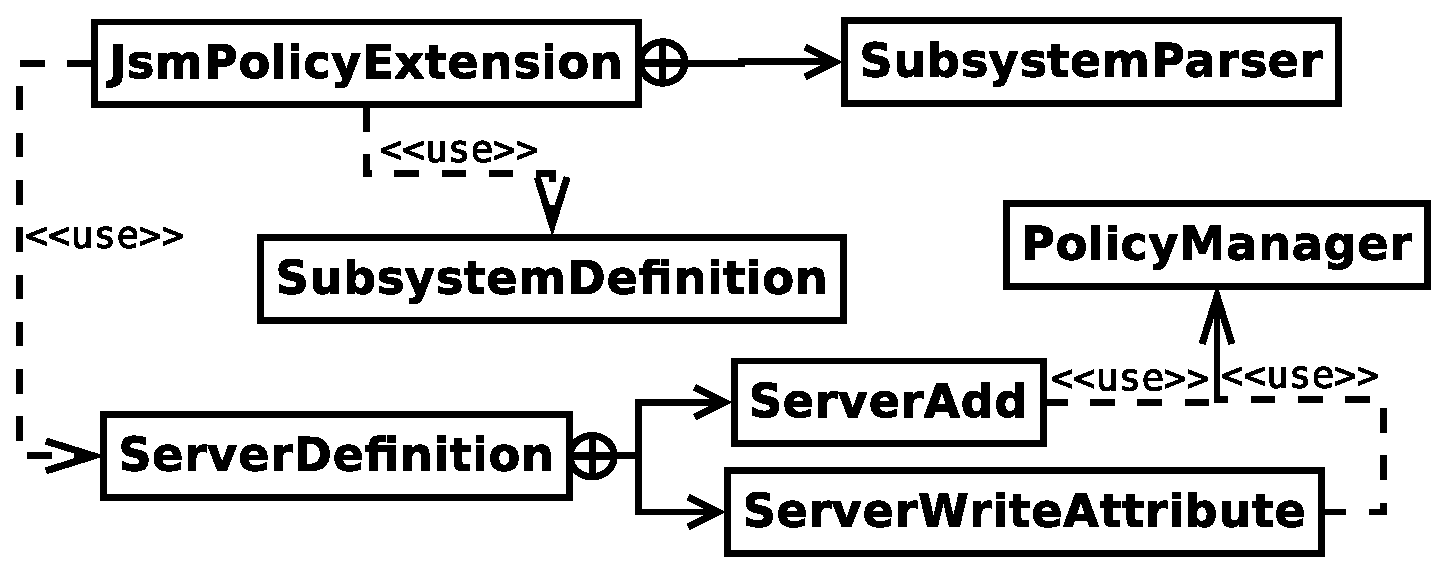
\includegraphics[width=10cm]{fig/tridy1}
  \caption{Diagram tříd prototypu}
  \label{tridy1}
\end{figure}

Byla tedy vytvořena třída definující rozšíření, {\tt JsmPolicyExtension}.
Její vnitřní třídou byla třída, zajišťující načítání a ukládání podstromu konfiguračního stromu patřící subsystému, {\tt SubsystemParser}.
Uzel {\tt subsystem=jsmpolicy} byl definován třídou {\tt SubsystemDefin ition} a uzel serveru ({\tt server=*}) třídou {\tt ServerDefinition}.
Oba uzly byly zaregistrovány jako součásti rozšíření {\tt JsmPolicyExtension}.

V~rámci konstruktoru třídy definující server bylo provedeno navázání akcí vytvoření serveru a odstranění serveru na třídy ošetřující tyto akce -- {\tt ServerAdd} a {\tt ServerRemove}.
V~rámci k~tomu určené metodě {\tt registerAttributes()} třídy definující uzel serveru byla zaregistrována konfigurační vlastnost {\tt policy}.
Zápis do této konfigurační vlastnosti byl ošetřen třídou {\tt ServerWriteAttribute}.
Těmito třídami bylo na operace nad uzly serveru a jejich vlastnostmi navázána akce nastavení dané bezpečnostní politiky.
Ta byla realizována třídní metodou {\tt setPolicy()} třídy {\tt PolicyManager}, zodpovídající za veškeré nastavování bezpečnostní politiky.
Bezpečnostní politika tak byla na server odpovídajícího názvu nasazována při vytvoření uzlu tohoto serveru, při změně obsahu jeho vlastnosti stanovující URL adresu k~souboru bezpečnostní politiky, a odebírána při odstranění tohoto uzlu.

\begin{figure}[tbh]
\begin{lstlisting}[caption=Metoda {\tt PolicyManager.setPolicy()} zajišťující nasazení souboru bezpečnostní politiky, label=setPolicyMethod]
public void setPolicy(String policy) throws OperationFailedException {
    if (policy == null) {
        System.setSecurityManager(null);
    } else {
        System.setProperty("java.security.policy", policy);
        refreshDelegatingPolicy(); // DelegatingPolicy.delegate.refresh()
        System.setSecurityManager(new SecurityManager());
    }
}
\end{lstlisting}
\end{figure}

Samotnou metodu {\tt setPolicy()}, zajišťující nasazení souboru bezpečnostní politiky, ukazuje ukázka kódu \ref{setPolicyMethod}.
Je-li jako parametr předána hodnota  {\tt null}, je správce bezpečnosti vypnut.
Je-li jako parametr předán platný řetězec, je použit jako URL adresa souboru bezpečnostní politiky -- je uložen do konfigurační proměnné {\tt java.security.policy}, je vyžádáno znovunačtení bezpečnostní politiky a jako správce bezpečnosti je nastaven standardní správce bezpečnosti Javy.

Samotné znovunačtení politiky přitom nemůže být provedeno pouhým voláním metody {\tt refresh()} používaného objektu bezpečnostní politiky.
Protože je jako jako objekt bezpečnostní politiky využíváno {\tt DelegatingPolicy}, je nutné toto metodu volat nad jeho privátní vlastností {\tt delegate},
jak je již popsáno v~kapitole \ref{zmenaZaBehu}. Metoda {\tt refreshDelegatingPoli cy()} zde svojí funkčností odpovídá ukázce kódu \ref{refreshDelegating}.

Subsystém v~této verzi žádným způsobem nezajišťoval distribuci souborů bezpečnostní politiky -- soubor musel být skrze uvedenou URL adresu přístupný ze serveru, na kterém měla být politika nasazena. V~opačném případě se nasazení bezpečnostní politiky nezdařilo.

%=============================================================================
\section{Konečná verze subsystému}
%=============================================================================

Konečná verze subsystému se od prototypu liší zejména tím, že v~konfiguračním stromu již nejsou ukládány jen URL adresy souborů politiky, ale také samotné soubory bezpečnostní politiky.

Byl tedy vytvořen další poduzel uzlu subsystému, {\tt policy=*}. Tento nový uzel představuje bezpečnostní politiku a jeho vlastností {\tt file} je obsah této politiky ve formě řetězce, tak jak by byl uložen v~souboru bezpečnostní politiky.
Zároveň byl změněn význam konfigurační vlastnosti {\tt policy} uzlu {\tt server=*}. Zatímco doposud obsahoval URL adresu souboru bezpečnostní politiky nasazené na daném serveru, nově obsahuje název uzlu {\tt policy=*}, jehož hodnota atributu {\tt file} má být použita jako obsah souboru bezpečnostní politiky pro daný server.

Nadále tak nestačilo provádět nasazení bezpečnostní politiky při změně atributu {\tt policy} uzlu {\tt server=*}, ale bylo nutné bezpečnostní politiku znovu nasadit také při změně obsahu vlastnosti {\tt file} uzlu {\tt policy=*}.

\begin{figure}[ht]
  \centering
  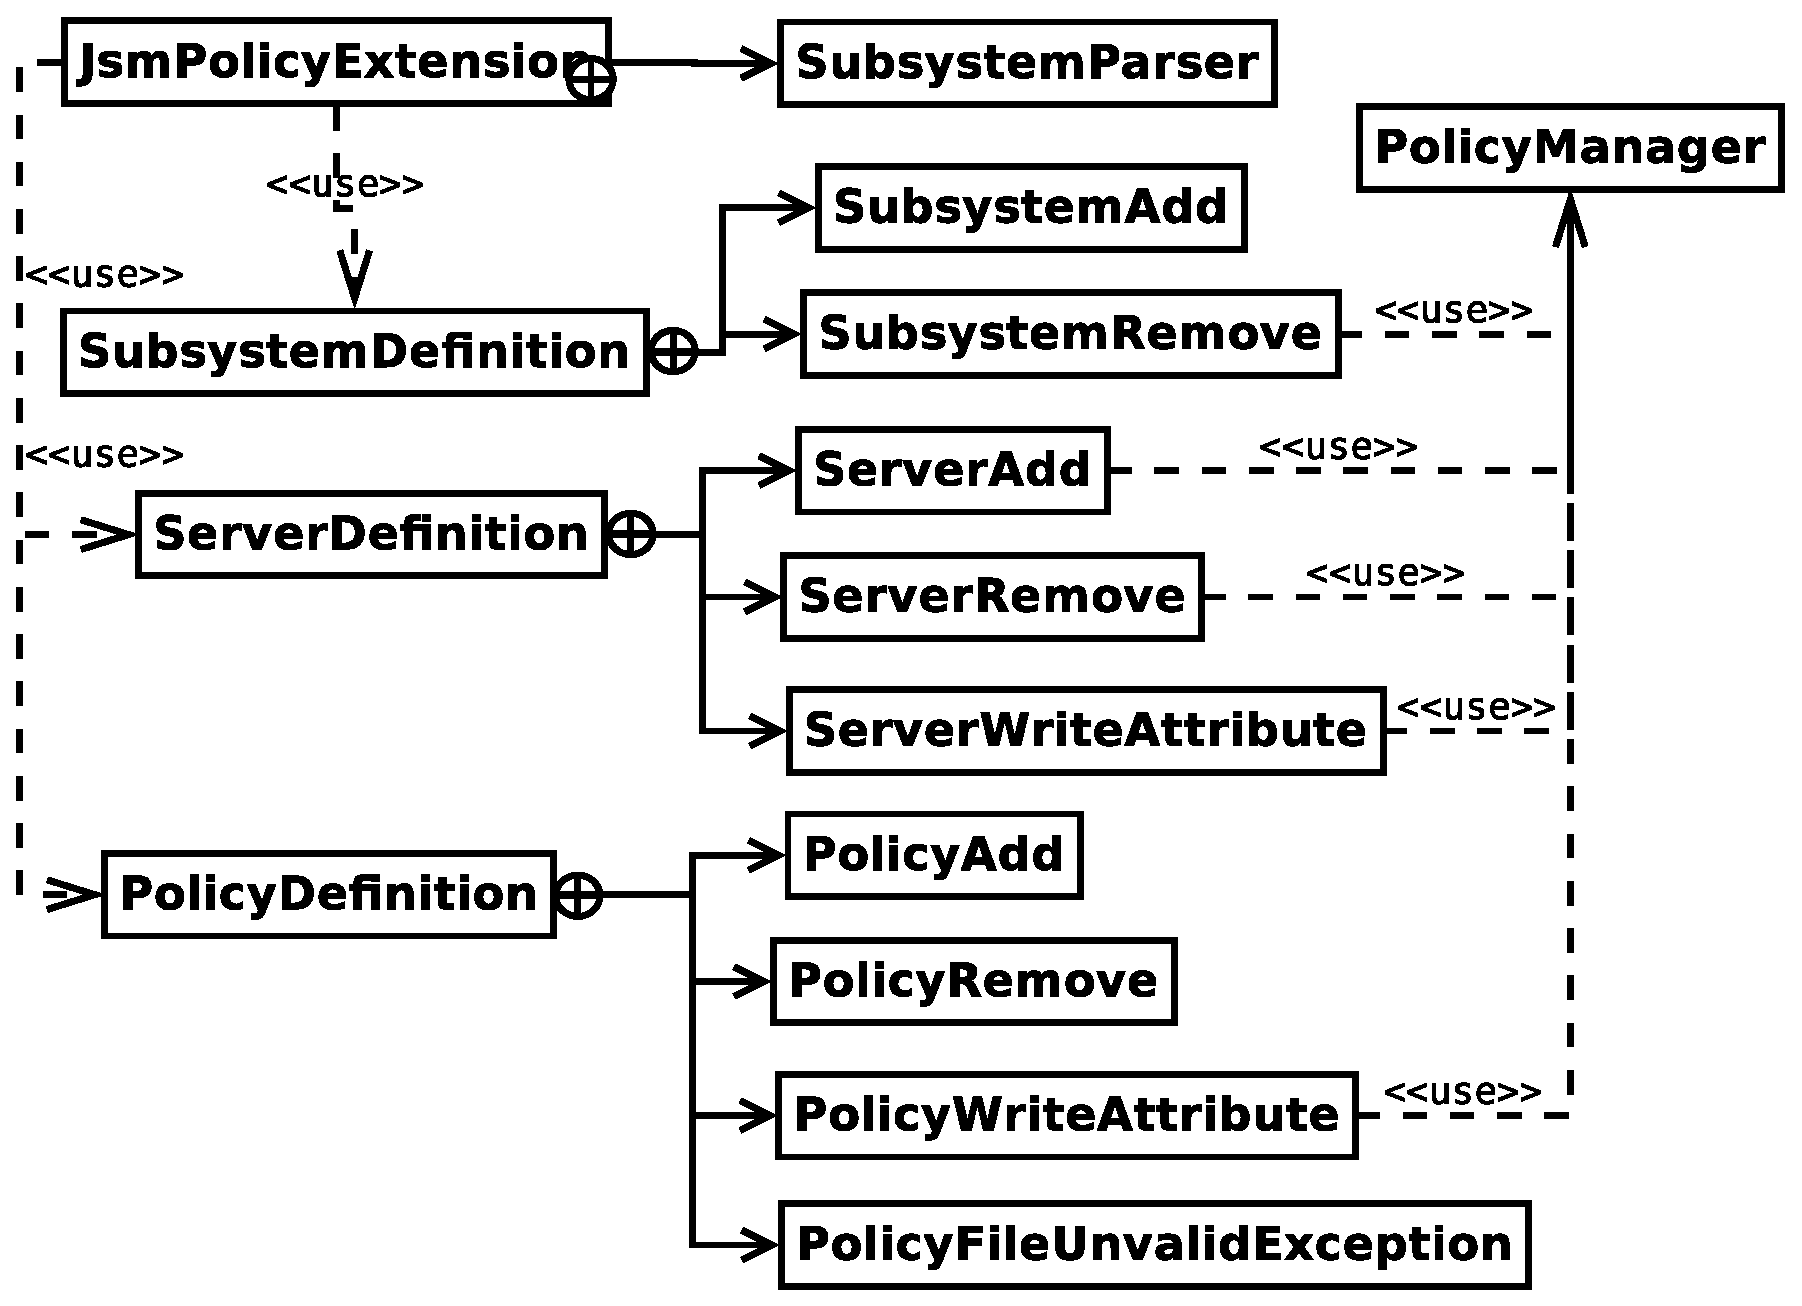
\includegraphics[width=12cm]{fig/tridy2}
  \caption{Diagram tříd konečné verze implementovaného rozšíření WildFly}
  \label{tridy2}
\end{figure}

Nasazování bezpečnostní politiky je řešeno analogicky jako v~případě akce navázané na změnu vlastnosti serveru -- třídou {\tt PolicyWriteAttribute} ošetřující zápis do konfigurační vlastnosti {\tt file}.
Při definici této konfigurační vlastnosti byl navíc definován také objekt validátoru -- objektu zajišťujícího kontrolu ukládané hodnoty konfigurační vlastnosti {\tt file}. Není-li hodnota platným souborem bezpečnostní politiky, je uložení odmítnuto. Tato kontrola je prováděna za pomoci třídní metody {\tt validatePolicyFile()} třídy {\tt PolicyManager}.
Aby bylo možné stejnou kontrolu provádět také při vytváření nového uzlu bezpečnostní politiky, musela být vytvořena třída {\tt PolicyAdd} ošetřující vytváření těchto uzlů.
Zároveň byla definována také třída {\tt Removepolicy} ošetřující operaci odstranění uzlu bezpečnostní politiky. Ta znemožňuje odstranění uzlu bezpečnostní politiky, která je aktuálně používána alespoň jedním serverem. (Existuje-li uzel serveru, jehož vlastnost {\tt policy} obsahuje název odstraňovaného uzlu {\tt policy=*}, není odstranění provedeno.)

\begin{figure}[tbh]
\begin{lstlisting}[caption=Klíčová část metody {\tt setPolicyFile()} třídy {\tt PolicyManager}, label=setPolicyFile]
public void setPolicyFile(String fileContent) throws OperationFailedException {
 if (fileContent == null) {
  setPolicy(null);
 } else {
  String tempDirString=System.getProperty("jboss.server.temp.dir",null);
  File tempDir = tempDirString == null ? null : new File(tempDirString);
  File temp = File.createTempFile("jsm-", ".policy", tempDir);
  FileOutputStream out = new FileOutputStream(temp);
  out.write(fileContent.getBytes());
  out.close();
  setPolicy(temp.getAbsolutePath()); // use temp file as policy file
  temp.delete();
 }
}
\end{lstlisting}
\end{figure}

Samotné nasazování bezpečnostní politiky zajišťuje metoda {\tt setPolicyFile()}. Její hlavní část zachycuje ukázka kódu \ref{setPolicyFile}.
Jak je vidět, k~samotnému nasazení bezpečnostní politiky využívá metodu {\tt setPolicy()} popsanou v~kapitole \ref{prototyp}.
Jejím vstupem však není adresa souboru bezpečnostní politiky, ale jeho obsah. Není-li roven {\tt null},
je vytvořen dočasný soubor {\tt jsm-*.policy} a obsah souboru bezpečnostní politiky ({\tt fileContent}) uložen do něj.
Dočasný soubor je jako soubor politiky nastaven metodou {\tt setPolicy()} popsanou v~kapitole \ref{prototyp} a smazán.
V~opačném případě, kdy je obsah bezpečnostní politiky roven {\tt null}, je rovněž volána metoda {\tt setPolicy()}, ale s~parametrem {\tt null}, čímž je používání bezpečnostní politiky a správce bezpečnosti vypnuto.

Jak je tedy vidět, používání souborů bezpečnostních politik uložených v~konfiguračním stromu WildFly tak je ve své podstatě triviální.

%%%%%%%%%%%%%%%%%%%%%%%%%%%%%%%%%%%%%%%%%%%%%%%%%%%%%%%%%%%%%%%%%%%%%%%%%%%%%%
\chapter{Testování systému} \label{testovani}
%%%%%%%%%%%%%%%%%%%%%%%%%%%%%%%%%%%%%%%%%%%%%%%%%%%%%%%%%%%%%%%%%%%%%%%%%%%%%%

Protože cílem této bakalářské práce nebylo jen vytvoření systému umožňujícího správu bezpečnostních politik nasazených na jednotlivých serverech distribuovaného systému, ale také prokázání jako kvality prostřednictvím testů, tato kapitola se zabývá tvorbou testů, umožňujících otestovat implementované řešení.

%=============================================================================
\section{Analýza} % na co testy delat
%=============================================================================

Cílem implementace řešení bylo umožnění nasazování bezpečnostní politik na servery v~doméně aplikačních serverů WildFly.
Implementované řešení by mělo být schopné nasadit bezpečnostní politiku na specifikovaný server na základě požadavku skrze JBoss Management API.
Testování by se tak jednoznačně mělo soustředit právě na schopnost systému nastavit na základě požadavku na stanoveném serveru stanovenou politiku.

Testování této klíčové vlastnosti je možné provádět jedině v~rámci testu integračního, tedy testu testujícího systém jako celek.
Jednotkové testování v~této oblasti sice rovněž může odhalit některé chyby, s~hledáním klíčových chyb, vyplývajících z~manipulací s~bezpečnostními politikami pod WildFly, však pomoci nemůže.

Integrační test pak bude založen na testování schopnosti uživatelské aplikace přistoupit k~souboru, k~němuž je přístup omezen bezpečnostní politikou a na vyměňování bezpečnostní politiky skrze testovaný subsystém v~průběhu testu.

Vzhledem k~tomu že nejsložitější možnou situací, která může v~rámci jednoho serveru nastat je výměna jedné bezpečnostní politiky za druhou,
k~úplnému otestování implementovaného řešení postačují dva testovací soubory a dvě testovací bezpečnostní politiky.
První bezpečnostní politika přitom bude přidělovat oprávnění přístupu pouze k~prvnímu souboru a druhá pouze k~druhému.

%=============================================================================
\section{Implementace testů} % popis implementacniho reseni
%=============================================================================

Implementované integrační testy jsou tvořeny dvěma částmi -- agentem a managerem.

{\bf Agent} je standardní uživatelskou Java EE aplikací nasazovanou na testovaný aplikační server. Na základě požadavku na rozhraní REST (Representational State Transfer) se pokusí přečíst požadovaný testovací soubor. Následně vrátí řetězec {\tt true} v~případě že se mu to podaří. V~případě že mu v~tom bezpečnostní politiky zabrání, vrátí řetězec {\tt false}.

{\bf Manager} je běžným JUnit testem. Na základě komunikace s~agentem prostřednictvím rozhraní REST zjišťuje, ke kterým testovacím souborům má agent oprávnění přistupovat. Skrze rozhraní JBoss Management API pak je schopný požádat subsystém nainstalovaný na serveru o~použití vybrané politiky na vybraný server.

Samotný test řídí Manager. Postupně žádá o~nasazení jednotlivých souborů bezpečnostní politiky a testuje, zdali má Agent oprávnění přistupovat ke správné podmnožině z~nich.

%=============================================================================
\section{Testovací prostředí} % popis popis runtime testovaciho prostredi
%=============================================================================

Implementované testy předpokládají doménu aplikačních serverů o~alespoň dvou WildFly serverech. Otestovanou verzí WildFly je 8.0.0.Final.
Názvy těchto serverů a URL adresy na kterých poskytují své služby je možné nastavit v~souboru {\tt manager/src/test/java/org/pic ketbox/jsmpolicy/test/Constants.java}. Na stejném místě je možné nastavit také adresu doménového řadiče a port na kterém poskytuje HTTP Management API.

Tyto servery mohou ale také nemusí být servery jediného hostitele. Na všech hostitelích ale již musí být nainstalováno implementované rozšíření a záplata zavaděče tříd modulů WildFly nastavená na používání dynamických bezpečnostních politik. Samotný subsystém nemusí být na jednotlivých serverech nasazen, bude nasazen automaticky v~rámci inicializace testu.

%=============================================================================
\section{Výsledky testování}
%=============================================================================

Všechny testy proběhly v~rámci závěrečného testování implementovaného řešení v~pořádku.
Byla-li na server nasazena bezpečnostní politika, byla účinná ihned po skončení provádění příkazu provádějícího její nasazení.
Byly-li na různé servery souběžně nasazovány dvě různé politiky, vzájemně se neovlivňovaly -- na první server je vždy aplikována jen politika určená pro první server a na druhý server jen politika určená druhému serveru.

%=============================================================================
\section{Zhodnocení}
%=============================================================================

Testování prokázalo, že implementovaný subsystém dokáže bez problémů nastavovat bezpečnostní politiky serverů domény, aniž by se přitom bezpečnostní politiky nasazené na různých serverech domény vzájemně ovlivňovaly.

Implementované řešení tedy dosáhlo cílů, které byly při jeho návrhu stanoveny.

%%%%%%%%%%%%%%%%%%%%%%%%%%%%%%%%%%%%%%%%%%%%%%%%%%%%%%%%%%%%%%%%%%%%%%%%%%%%%%
\chapter{Závěr}
%%%%%%%%%%%%%%%%%%%%%%%%%%%%%%%%%%%%%%%%%%%%%%%%%%%%%%%%%%%%%%%%%%%%%%%%%%%%%%

Cílem práce bylo navrhnout, vytvořit a otestovat systém pro centralizovanou správu a distribuci bezpečnostních politik Javy v~distribuovaném prostředí aplikačního serveru WildFly.
Ačkoli jen samotné používání bezpečnostní politiky ve WildFly bylo v~době tvorby této práce bez znalosti zdrojového kódu nemožné (viz kapitola \ref{jboss}),
byl v~rámci této bakalářské práce nejen nalezen způsob jak bezpečnostní politiky ve WildFly používat, ale také vytvořen nový způsob, umožňující také její výměnu za běhu aplikačního serveru bez potřeby jeho restartu nebo znovunačtení.

Dosaženo toho bylo za pomoci vytvořené záplaty (patch) WildFly (viz kapitola \ref{upravaZavadeceWildFly}), která byla zároveň předána
k~začlenění do hlavní vývojové větve. \cite{jmPullRequest}
Po vyřešení samotného používání a výměny bezpečnostních politik v~prostředí aplikačního serveru WildFly bylo vytvořeno rozšíření aplikačního serveru.
To umožňuje provádět výměnu používané politiky a zapínat/vypínat správce bezpečnosti v~návaznosti na změnu konfigurace pro příslušný server
v~konfiguračním stromu WildFly.
Konfigurační strom WildFly se zároveň používá také pro ukládání jednotlivých souborů bezpečnostní politiky, které jsou tímto způsobem distribuovány napříč aplikačními servery domény.

Nad tímto rozšířením aplikačního serveru pak bylo vytvořeno webové uživatelské rozhraní ve formě rozšíření webové administrační konzoly WildFly.
To umožňuje nastavovat použití správce bezpečnosti a nastavovat bezpečnostní politiky na jednotlivých serverech nebo celých skupinách serverů WildFly domény.

Na implementované řešení byla nakonec vytvořena automatizovaná sada testů, umožňující otestovat schopnost implementovaného systému měnit oprávnění
aplikací nasazených na aplikačním serveru nebo v~doméně aplikačních serverů.

Možným vylepšením implementovaného řešení do budoucna by mohlo být umožnění nasazování bezpečnostních politik na celé skupiny aplikačních serverů ne na úrovní webové administrační konzoly WildFly, ale již na úrovni JBoss Management API. Uživatel by tak mohl provádět nasazování politik na skupiny serverů vlastním skriptem bez potřeby procházení jednotlivých serverů skupiny na úrovni tohoto skriptu.

Rozsáhlejším možným rozšířením implementovaného systému by pak mohl být zadávání bezpečnostních politik, již ne ve formě textu v~syntaxi typické pro bezpečnostní politiky uložené v~textových souborech, ale prostřednictvím uživatelského rozhraní.
To by mohlo umožnit zadávat bezpečnostní politiku po jednotlivých oprávněních a za pomoci omezených nabídek, tedy s~mnohem menším rizikem zadání neplatné politiky oproti implementovanému řešení, kde se uživatel dozvídá o~neplatnosti zadané politiky až při jejím uložení.

%Byly splněny všechny cíle stanovené zadáním práce. Úvahu, nakolik výsledky této práce prospějí budoucímu vývoji aplikačního serveru WildFly, ponechám na čtenáři.

